\documentclass[11pt,norsk,a4paper]{article}
%%%%%%%%%%%%%%%%%%%%%%%%%%%
% MonKey bachelors thesis %
%%%%%%%%%%%%%%%%%%%%%%%%%%%

%%%%%%%%%%%%%%%%%%%%%%%%%%%%
% LINE SPACING
\newcommand{\linespacing}{1.5}
\renewcommand{\baselinestretch}{\linespacing}
%%%%%%%%%%%%%%%%%%%%%%%%%%%%


\usepackage[utf8]{inputenc}     % For utf8 encoded .tex files
\usepackage[absolute]{textpos}
\usepackage[T1]{fontenc}
\usepackage{cite}
\usepackage{listings,babel,graphicx,mathpple,textcomp,varioref,pdfpages,geometry} % For inclusion of graphics
\usepackage[toc,page]{appendix}
\usepackage[flushleft]{threeparttable}
\usepackage{fancyhdr}
\pagestyle{fancy}
\usepackage{color}

\geometry{a4paper, top=1.5cm, left=2.5cm, right=3.0cm, bottom=2.0cm, includehead, includefoot}

\definecolor{mygreen}{rgb}{0,0.6,0}
\definecolor{mygray}{rgb}{0.5,0.5,0.5}
\definecolor{mymauve}{rgb}{0.58,0,0.82}

% xleftmargin=17pt, framexleftmargin=17pt, framexrightmargin=5pt, framexbottommargin=4pt
%basicstyle=\footnotesize
%captionpos=b		cation on bottom
%numbersep=5pt
%stepnumber=2		noclue
\lstset{ 
backgroundcolor=\color{white}, 
basicstyle=\scriptsize, breakatwhitespace=false, 
breaklines=true, commentstyle=\color{mygreen}, 
deletekeywords={...}, escapeinside={\%*}{*)}, 
extendedchars=true, frame=single, keywordstyle=\color{blue}, 
language=Octave, morekeywords={*,...}, numbers=left, 
numbersep=5pt, stepnumber=1, numberstyle=\tiny\color{mygray}, 
rulecolor=\color{black}, showspaces=false, showstringspaces=false, 
showtabs=false, stringstyle=\color{mymauve}, tabsize=2, title=\lstname, 
xleftmargin=3em, framexrightmargin=5pt, framexbottommargin=4pt 
}

%%%%%%%%%%%%%%%%%%%%%%%%%%%%
% HYPERREF
\usepackage[colorlinks,pagebackref,pdfusetitle,urlcolor=blue,citecolor=blue,linkcolor=blue,bookmarksnumbered,plainpages=false]{hyperref}
% For print version, use this instead:
%\usepackage[pdfusetitle,bookmarksnumbered,plainpages=false]{hyperref}
%\usepackage{backref}
%\renewcommand{\backrefpagesname}{Cited on}
%%%%%%%%%%%%%%%%%%%%%%%%%%%%

\newcounter{includepdfpage}
\newcounter{currentpagecounter}
\newcommand{\addlabelstoallincludedpages}[1]{
   \refstepcounter{includepdfpage}
   \stepcounter{currentpagecounter}
	\appendix
   \label{#1.\thecurrentpagecounter}}
\newcommand{\modifiedincludepdf}[3]{
    \setcounter{currentpagecounter}{0}
    \includepdf[pages=#1,pagecommand=\addlabelstoallincludedpages{#2}]{#3}}


\newenvironment{changemargin}[2]{%
\begin{list}{}{%
\linespread{0.9}% linespace between code
\setlength{\topsep}{0pt}%
\setlength{\leftmargin}{#1}%
\setlength{\rightmargin}{#2}%
\setlength{\listparindent}{\parindent}%
\setlength{\itemindent}{\parindent}%
\setlength{\parsep}{\parskip}%
}%
\item[]}{\end{list}}

\newcommand{\HRule}{\rule{\linewidth}{0.5mm}}

\title{Rapport, Monitoring is Key}
\author{Øyvind Sigerstad, Nils Slåen og Bjørn-Erik Strand}

\tolerance = 5000
\hbadness = \tolerance
\pretolerance = 2000

\begin{document}

\begin{titlepage}
\begin{center}

% Upper part of the page. The '~' is needed because \\
% only works if a paragraph has started.

\includegraphics[width=0.50\textwidth]{higlogo}~\\[1cm]

\textsc{\LARGE Høgskolen i Gjøvik}\\[1.5cm]

\textsc{\Large Rapport}\\[0.5cm]

% Title
\HRule \\[0.4cm]
{ \huge \bfseries MonKey}\\[0.4cm]
{ \large \emph{"Monitoring is Key"}} \\ [0.3cm]
\HRule \\[1.5cm]

% Author and supervisor
\begin{minipage}{0.4\textwidth}
\begin{flushleft} \large
\emph{Av:}\\
Øyvind Sigerstad\\
Nils Slåen\\
Bjørn-Erik Strand
\end{flushleft}
\end{minipage}
\begin{minipage}{0.4\textwidth}
\begin{flushright} \large
\emph{Veileder:} \\
Erik Hjelmås
\end{flushright}
\end{minipage}

\vfill

% Bottom of the page
{\large \today}

\end{center}
\end{titlepage}
\fancyhead[R]{\small MonKey - Monitoring is Key}
\pagenumbering{roman}

%%%%%%%%%%%%%%%%%%%%%%%%%%%%
% DECLARATIONS
\chapter{Forord}
	Takk til:
    Veileder Erik Helmås
    Hele IKT-avdelingen i Hedmark fylkeskommune
    Bachelorgruppen dot11ac
    IT tjenesten HiG ved Jon langset for presentasjon
    dnsmichi @ icinga dev team

% ADDITIONAL DECLARATIONS HERE (IF ANY)

%%%%%%%%%%%%%%%%%%%%%%%%%%%%

%%%%%%%%%%%%%%%%%%%%%%%%%%%%
% SUMMARY PAGE
%\thispagestyle{empty}
\newpage
%\null\vskip10mm
\begin{center}
\large
\underline{UNIVERSITY OF SUSSEX}
\vskip20mm
% AUTHOR, QUALIFICATION
%\textsc{Joe Bloggs, Doctor of Philosophy}
\vskip20mm
% TITLE
\underline{\textsc{My Theory of Everything}}
\vskip0mm
% SUBTITLE (optional)
\underline{\textsc{How it all works}}
\vskip20mm
\underline{\textsc{Summary}}
\vskip2mm
\end{center}
% Change line spacing
%\renewcommand{\baselinestretch}{1.0}
\small\normalsize
% SUMMARY HERE (300 word limit for most subjects):

%%%%%%%%%%%%%%%%%%%%%%%%%%%%

%%%%%%%%%%%%%%%%%%%%%%%%%%%%
% ACKNOWLEDGEMENTS
\chapter*{Acknowledgements}
yeeah boy
%\renewcommand{\baselinestretch}{\linespacing}
\small\normalsize
% ACKNOWLEDGEMENTS HERE:

%%%%%%%%%%%%%%%%%%%%%%%%%%%%


%%%%%%%%%%%%%%%%%%%%%%%%%%%%
% TABLE OF CONTENTS, LISTS OF TABLES & FIGURES
\newpage
%\pdfbookmark[0]{Contents}{contents_bookmark}
\tableofcontents
\listoftables
%\phantomsection
%\addcontentsline{toc}{chapter}{List of Tables}
\listoffigures
%\phantomsection
%\addcontentsline{toc}{chapter}{List of Figures}
%%%%%%%%%%%%%%%%%%%%%%%%%%%%

%%%%%%%%%%%%%%%%%%%%%%%%%%%%
% MAIN THESIS TEXT: arabic page numbering 1, 2, 3, ...
\newpage
\pagenumbering{arabic}
%%%%%%%%%%%%%%%%%%%%%%%%%%%%

\chapter{Innledning}
\section{Bakgrunn}
Serviceenheten IKT ved Hedmark Fylkeskommune (heretter kalt IKT-avdelingen) har det overordnede ansvaret for alt datautstyr som tilhører fylkeskommunen og datanettverket for sentraladministrasjonen og øvrige lokasjoner. Dette omfatter blant annet videregående skoler, tannklinikker, Hedmark Trafikk m.fl. Totalt benyttes IT-løsningene av over 10 000 brukere.

Datasystemene er kritiske for daglig drift av de mange funksjonene fylkeskommunen har. Det er derfor mange brukere som berøres dersom en feil skulle inntreffe i systemene. Det er viktig at de ansvarlige får beskjed så raskt og effektivt som mulig når et system går ned eller ikke fungerer som det skal.

Per i dag benyttes et enkelt overvåkningssystem, “Servers Alive”, \cite{servers}, som ikke dekker IKT-avdelingens behov. Oppsettet gir for mye irrelevant informasjon, som gjør at en ikke får et godt nok oversiktsbilde. Det mangler også mulighet for å kunne overvåke mange ønskede parametere. Systemet gir kun varsling til skjerm, og det er ønskelig å også kunne få SMS og e-post. Det er også en proprietær løsning og dermed ikke lett å utvide. I tillegg til dette kjøres ikke sjekkene parallelt, og derfor skalerer systemet dårlig.

IKT-avdelingen har lenge arbeidet med å finne en bedre overvåkningsløsning for infrastrukturen enn dagens. Det er ønskelig å erstatte denne løsningen med en mer modulbasert, der IKT-avdelingen har tilgang til kildekoden og kan utføre endringer.

De har imidlertid for hver runde konkludert med at de ikke har de nødvendige ressursene til å sette i gang et slikt prosjekt. Da vi forespurte IKT-avdelingen om de hadde noen mulige bachelorprosjekter, var de veldig interessert i at en bachelorgruppe kunne ta tak i denne problemstillingen.

\section{Oppgavebeskrivelse}
Det skal settes opp et overvåkningssystem som skal varsle feil og hendelser på enheter i fylkeskommunes datanettverk. Dette innebefatter servere med tjenester, og nettverksenheter som switcher, routere og brannmurer. Dette systemet må være modulært med mulighet for å enkelt kunne legge til nye moduler i ettertid. Følgende krav er satt til løsningen:

\begin{itemize}
	\item Webgrensesnitt for visning av overvåking på skjerm.
	\item Varsling av flere grader kritisk nivå. Med mulighet for varsling til SMS, e-post og skjerm.
	\item Avhengigheter mellom enheter som overvåkes skal kunne settes opp. Varsling skal gi informasjon om det er antatt følgefeil og hovedfeil.
	\item Systemet skal ta høyde for redundante systemer.
	\item Alle hendelser skal logges og lagres i database.
	\item Støtte WMI, SNMP, ICMP (med antall drop før varsling), og evt. andre aktuelle standarder.
	\item Det skal være enkelt å legge til nye enheter for overvåking.
	\item Servermiljø skal kunne overvåkes på kjøling, temperatur, luftfuktighet og UPS.
\end{itemize}

Vi må derfor finne programvare som kan tilpasses fylkeskommunes systemer og dekker flest mulig av disse kravene. Dersom eksisterende løsninger ikke finnes, eller ikke dekker behovet, må vi utvikle dette selv.

IKT-avdelingen har også en liste over moduler de ønsker implementert i løsningen. Disse vil vi prøve å implementere dersom vi får tid.

\begin{itemize}
	\item Rapporter - Uthenting av trender, dagens situasjon osv.
	\item Driftsarbeid - Planlagt arbeid definert mot enheter vil ikke utløse alarm, men driftsarbeidsvarsling.
	\item SLA
	\item Vise SLA avtaler opp mot faktiske verdier.
	\item Kundebase med krav opp mot logget data.
	\item Kapasitetsmålinger opp mot maksverdier (f.eks. linjekapasitet).
	\item Dashboard-funksjonalitet med mulighet for personliggjøring av eget grafisk grensesnitt.
	\item Eget grensesnitt for mobile enheter.
	\item Konfigurasjonskart - Tegner kart av løsning grafisk med klikkbare objekter.
	\item CMDB - Mulighet for lagring av konfigurasjonsoppsett av objekter (enheter).
	\item Telefoni - Overvåking av telefonlinjer opp mot Trio og Asterisk.
\end{itemize}

\section{Avgrensninger}
Siden vi har både må-krav og ønsket-krav til funksjonalitet, må vi avgrense oss slik at vi overholder tidsrammer i forhold til må-krav. Om vi ser at vi ligger foran tidsskjema og har fått på plass alle må-kravene til implementasjonen, vil vi begynne å se på ønsket funksjonalitet.

\section{Målgruppe}
Overvåkningsløsningen utvikles for IKT-avdelingen, og ansatte her vil være en av målgruppene. Selve rapporten vil vinkles slik at sensor, medstudenter, veileder, oppdragsgiver og ellers andre interesserte kan få et innblikk i hvordan prossessen med å implementere en open source overvåkningsløsning har vært. Det faglige nivået på rapporten vil legges slik at medstudenter skjønner og kan lære noe av stoffet.

\section{Prosjektmål}
\subsubsection{Effektmål}
I forhold til dagens løsning skal den nye løsningen:
\begin{itemize}
	\item være mer oversiktlig.
	\item tilrettelegge for mer omfattende overvåkning.
	\item være mer fleksibel.
	\item bidra til mer effektiv drift for IKT-avdelingen, der hendelser raskt kan oppdages og eskaleres.
\end{itemize}

\subsubsection{Resultatmål}
\begin{itemize}
	\item Utvikle en overvåkningsløsning som tilfredsstiller de krav som er satt.
	\item Den nye overvåkningsløsningen vil resultere i at den eksisterende kan erstattes og deretter fases ut.
\end{itemize}

\subsubsection{Læringsmål}
\begin{itemize}
	\item Sette oss inn i “best practices” for overvåking av datasystemer.
	\item Kunne tilpasse og implementere en overvåkningsløsning for små og mellomstore bedrifter.
\end{itemize}

\section{Rammer}
Følgende krav er gitt i oppgaven:
\begin{itemize}
	\item Dersom eksisterende programvare benyttes må denne være open source.
	\item MySQL skal benyttes som databasesystem.
	\item Prosjektrapporten skal ikke inneholde sensitiv informasjon om Hedmark fylkeskommunes tekniske løsninger. Eksempelvis IP-adresser, brukernavn/passord og brannmurkonfigurasjon. Dette er i tråd med taushetserklæringen som må inngås.
	\item Det skal kjøpes inn en enhet for å overvåke luftfuktighet og temperaturer. Innkjøp av denne skal skje i henhold til fylkeskommunens innkjøpsrutiner.
\end{itemize}

\section{Faglig bakgrunn}


Bjørn-Erik og Øyvind er 3. års studenter på Drift av nettverk og datasystemer, mens Nils går 3. året på Dataingeniør. Gjennom to og et halvt år på Høgskolen i Gjøvik har vi tatt fag innenfor programmering, nettverk, databaser, sikkerhet og forskjellig grad av matematikk, inkludert statistikk. Nils og Øyvind har tidligere vært lærlinger ved henholdsvis Hedmark Fylkeskommune og Hamar Katedralskole der de fikk kunnskap om deres applikasjoner og infrastruktur.

Bjørn-Erik og Øyvind har også tidligere skrevet en rapport om bruk av ITIL ved Hedmark fylkeskommunes IKT-avdeling i faget “IT Service Mangement”.

En overvåkningsoppgave med denne oppgavebeskrivelsen følte vi hadde potensiale til å komme innom de fleste temaene vi har vært innom gjennom studiet. Her er det også områder der gruppen har delvis eller manglende kunnskap, både om hvilke teknologier som finnes og hvordan vi bruker disse i et større datamiljø.

\section{Roller}
\subsubsection{Prosjektleder}
Prosjektleder vil være Øyvind Sigerstad. Denne rollen vil være fast under hele prosjektet. Lederens hovedansvar er å se nødvendigheten for møter, samt ha et overordnet ansvar for arbeidsfordelingen. Prosjektlederen vil også ta endelige avgjørelser dersom gruppen ikke kan komme til enighet, som stipulert i gruppereglene.

\subsubsection{Kommunikasjonsansvarlig}
Vår kontaktperson er Nils Slåen. All kontakt med oppdragsgiver og annen utgående kommunikasjon vil gå via ham. Kommunikasjonsansvarlig har også ansvar for å avtale møter.

\subsubsection{Webansvarlig}
Vår webansvarlig er Bjørn-Erik Strand. Hans hovedansvar er å sette websiden vår i drift før fristen. Webansvarlig har også et overordnet ansvar for å få oppdateringer publisert. De andre medlemmene i gruppen skal også ha tilgang til å utføre oppdateringer.

\subsubsection{Oppdragsgiver}
Vår oppdragsgiver er Svein-Inge Kvalø (Fungerende driftsleder ved IKT-avdelingen, Hedmark fylkeskommune). Han er vårt kontaktpunkt ved Hedmark fylkeskommune. Lasse Odden er vår tekniske kontakt (IT-konsulent ved IKT-avdelingen - Hedmark fylkeskommune). Han vil være en ressurs vi kan bruke om vi lurer på noe teknisk ved IKT-avdelingens eget oppsett.

\subsubsection{Veileder}
Erik Hjelmås (Førsteamanuensis, Dr. scient ved HiG), er vår veileder gjennom bacheloroppgaven.

\section{Rutiner og regler i gruppa}
Et eget dokument er utarbeidet med grupperegler som alle gruppens medlemmer er enige i og har skrevet under på. Dette finnes under som vedlegg xxx.

\section{Verktøy}
Alt av egenutviklet kildekode og konfigurasjonsfiler vil bli lagt under et SVN repository. Dette for å få versjonskontroll og samle alt på et sted, som vi kan ta backup av. Google Docs vil bli brukt for å enkelt kunne samarbeide på dokumenter. Når den endelige rapporten skal genereres, vil vi importere Google Docs-dokumentet til LaTeX. Dropbox vil bli benyttet til å dele filer og dokumenter innad i prosjektgruppen, og med oppdragsgiver. Vi vil bruke Wordpress som publiseringsverktøy for hjemmesiden.

Av andre verktøy har vi benyttet Microsoft Visio til å lage illustrasjoner. Grafene er generert av Graphite.

\section{Utviklingsmodell/rammeverk}
For å tilpasse overvåkningssystemet til IKT-avdelingens krav, vil det med stor sannsynlighet komme endringer etterhvert. Det vil kunne oppstå ulike situasjoner som er vanskelige å forutse. Eksempler på dette er at en plugin som kreves ikke eksiterer, webgrensesnittet må endres på grunn av mer informasjon eller omorganisering, eller oppdragsgiver har innspill som fører til endring av funksjonalitet i ettertid. Dette fører til at vi må ha en fleksibel modell med tanke på endringer og tilbakefall, men med begrensninger på hvor mye tid vi kan bruke ved uforutsette problemer.

På grunn av en naturlig sammenheng og avhengigheter mellom kravene som er satt, har vi valgt å gruppere funksjonalitet i moduler. De forskjellige modulene er “Kjerneprogramvare”, “Server”, “Infrastruktur”, “Servermiljø”, “Varsling” og “Statusvindu” (visualisert i punk x.x). Med nærliggende sammenheng mener vi at funksjonalitet som CPU, RAM, disk og prosesser er i samme kategori. Planen er også å gjennomføre disse i en gitt rekkefølge. Varsling kan settes opp uten noe input, men med tanke på redundans i systemene, avhengigheter mellom objektene, og testing av funksjonene som går inn under varsling, ser vi på dette som en avhengighet av “Server” og “Infrastruktur”. “Statusvindu” har vi valgt å legge sist fordi vi ser for oss at modulene “Server”, “Infrastruktur, “Servermiljø”, og “Varsling” må være på plass før en varslingsskjerm kan ferdigstilles.

I tradisjonell systemutvikling må man definere alle parametere og rekkefølge på alt som skal utvikles, før en starter med selve utviklingen. En smidig modell vil gi oss mer frihet til å gjøre justeringer underveis. Vi har derfor valgt en iterativ modell\cite{wiki:iterativ}. En del av den iterative modellen er “product control list”, men denne har vi valgt å ikke ta med fordi vi har satt opp en overordnet kategorisering av funksjonalitet, og bestemt når hver av disse skal implementeres.

Vi vil dele inn prosjektet i faser, som hver består av en planleggingsfase, en implementeringsfase, og en fase for testing og evaluering. Disse vil så gjentas for hver modul som skal implementeres. Halvveis i hver iterasjon vil vi ha et møte med oppdragsgiver der vi kan presentere funksjonalitet i modulen, og få tilbakemeldinger. Det gjør at vi kan jobbe med dette i den siste halvdelen av iterasjonen. Dette vil forhåpentligvis føre til at produktet ikke sporer av fra de forventningene og behovene IKT-avdelingen har.

%yo dudes!\ref{gen.bash}
%yo again dudes! \ref{ad_sync.pl}
%\\
%reftest2 \\
%yo doodsters \ref{opplaering}
%yo dood \ref{kartlegging}
%ja sann kan det gaaaa\cite{servers}

\chapter{Teori}
I dette kapittelet gjennomgås teori og konsepter som er nødvendig å forstå før implementasjonsdelen. Alternativer til kjerneprogramvare presenteres og valg av arkitektur gjennomgått.
\clearpage
\section{Hvorfor overvåke}
Nesten alle bedrifter i dag bruker IT-systemer for å gjøre seg mer effektiv og konkurransedyktig i markedet. Mange av disse systemene blir ofte tatt for gitt, fordi de rett og slett bare fungerer. Men hva skjer om e-posten en dag ikke virker, eller månedens lønn ikke kommer når den skal? I slike tilfeller kan en overvåkningsløsning være viktig for å oppdage og identifisere problemet tidlig.

Der en har avtaler knyttet til IT-tjenestene som blir levert, kan et overvåkningssystem være med på å dokumentere at tjenestene har vært i henhold til SLA. Overvåkning kan også bidra til å gi et bedre bilde på hvor pålitelige systemer og utstyr er, og kan hjelpe til med å kartlegge hvor systemene er sårbare. Dette kan igjen benyttes ved kapasistetsplanlegging. For de ansatte ved en driftsavdeling kan det også skape en trygghetsfølelse å vite at systemer overvåkes, og feil vil varsles.

Når en leverer tjenester innenfor IT er det viktig at det ikke er kunden som varsler om feilen. Da ender kundene opp som overvåkningsmekanismen. Kriteriene for varsling må være finjustert, slik at en kan reagere før systemene krasjer.

%I "The Practice of System and Network Administration"sier forfatteren det godt: 
\epigraph{``If you aren’t monitoring it, you aren’t managing it.''}{--- \textup{Limoncelli, Hogan \& Chalup }, The Practice of System and Network Administration\cite{practiceofsystemandnetwork}}

\section{Generelt om overvåkning}\label{sec:omovervakning}
Overvåkning deles ofte inn i kategoriene historisk overvåkning og sanntidsovervåkning. Ved historisk overvåkning blir data samlet inn for å ha statistikk om oppetid, ytelse og bruk. Ut fra disse dataene kan en trekke konklusjoner, som for eksempel at VPN-tjenesten har hatt en oppetid på 99,9 \% over det siste året og at gjennomsnittlig antall brukere har vært 100, med en økning på 10 \% den siste måneden. Dermed kan en få et overblikk over hvor mye nedetid tjenesten har hatt, og en har dokumentasjon på hvordan leveransen har vært opp mot avtalt leveranse.\cite{practiceofsystemandnetwork}

Ved å se på stigningstallet kan en også forsøke å si noe om trenden og forventet fremtidig nivå, som kan gi en indikasjon på nødvendige skaleringstiltak. For eksempel at med dagens bruk av toner på kopimaskinen, vil den gå tom for toner innen fredag. 

Sanntidsovervåkning vil si at en sjekker tilstanden til en enhet eller tjeneste i et gitt intervall, og så fort noe avviker fra normalen sendes det ut varsel. Målet er at de ansvarlige skal kunne vite om noe er feil så fort som mulig, og helst før brukerne.

\subsection{Overvåkning i ITIL}
ITIL (Information Technology Infrastucture Library) er et sett med standarder og konsepter som beskriver hvordan IT-tjenester kan kvalitetsikres innenfor leveranse, drift og support. ITIL brukes i dag av IT-bedrifter over hele verden og gir et felles rammeverk for hvordan en bør praktisere innen IT-sektoren. ITIL blir definert i et sett med bøker som blir utgitt av Office of Government Commerce i Storbritannia.

Innenfor ITIL er prossessflyt og involvering av ulike prosesser ved hendelser essensielt. Overvåkning av systemer og infrastruktur bak forretningskritiske systemer, og overvåkning av forretningskritiske systemer i seg selv er viktig i ITIL-prosessen Service Operations. Overvåkning og varsling er et viktig ledd for kunne å registrere en hendelse som kan være et engangstilfelle, eller en indikasjon på et underliggende problem. Et eksempel her vil være om en bruker melder inn at det er problem med innlogging på en terminalserver. Her kan et engangstilfelle være at passordet har løpt ut for denne brukeren, eller indikere et underliggende problem med LDAP-autentisering.

Når en hendelse inntreffer, enten ved at en bruker rapporterer om en feil eller at overvåkningsløsningen varsler om det, vil servicedesk være første instans som må reagere. Servicedesk er derfor et viktig ledd for å opprettholde forretningskritisk funksjonalitet, og en god statusvisning og tilrettelagt varsling vil bidra til å raskt identifisere hendelsen.

Overvåkning er også en del av komponenten ``Capacity Management'' innenfor kategorien ``Service Delivery'', som legger retningslinjer for proaktive handlinger framfor reaktive. Proaktive handlinger innebærer å være i forkant av hendelser som kan oppstå, og ikke reagere når det allerede har skjedd; reaktivt. Informasjon fra overvåkningen kan hjelpe til med å identfisere situasjoner som kan håndteres før hendelser inntreffer og får innvirkning for brukere. \cite{itil1,itil2,events}

\subsection{Hvordan overvåke}
Den enkleste formen for overvåkning av en server er å sende en ICMP echo request (ping), og se om en får et svar (også kjent som pong). En måler tiden til en får et svar tilbake, og sjekker hvor mange prosent av antall forsøk en får svar på. Dette betyr at enheten som kontaktes har en delvis fungerende IP-stack og om linjen imellom fungerer. Men det forteller ikke noe om tjenestene som kjører. Det er tross alt tjenestene som kjører på enheten som er grunnen til at en trenger enheten i utgangspunktet.

En bedre løsning er å teste hver av tjenestene. For en webserver kan det være å prøve å hente ned forsiden av hjemmesiden som skal leveres og sjekke at en får reponsen ``HTTP OK 200''. Da vil en vite at webserveren kjører og leverer ut sider riktig. Et skritt videre kan være å sjekke at siden inneholder riktig informasjon og at det ikke har blitt endret av uvedkommende (defacing).

\clearpage
\section{Hvilke overvåkingsløsninger finnes}\label{sec:hvilkefinnes}
Det finnes i dag mange løsninger for overvåkning av IT-systemer\cite{wiki:networkmonitoring}. Det ble tatt utgangspunkt i prosjektets rammer og krav til funksjonalitet, og valgt ut noen løsninger som ble undersøkt nærmere. Punktene om ønsket tilleggsfunksjonalitet ble også vektlagt slik at de skulle være lettere å implementere i senere faser av prosjektetet, eller i senere prosjekter. 

Det ble også gjort en gjennomgang med oppdragsgiver, hvor de ulike løsningene ble diskutert (presentasjon av dette ligger i Vedlegg \ref{app:presentasjoner}). De overvåkningsløsningene som ble vurdert nærmere etter den første runden med research er alle fri programvare og har en utbredt brukermasse. 
\begin{description}
\item[Zenoss] har en open source-lisens på Zenoss Core. Zenoss brukes av mange store aktører\cite{zenoss}, som gjorde denne til en mulig kandidat. Det ble likevel valgt å ikke bruke Zenoss på grunn av vinklingen de har mot ``Enterprise Solutions''\cite{zenpacks}. Dette involverer at en må kjøpe tilleggsmoduler til selve kjernen for å oppnå en komplett overvåkningsløsning.

\item[Observium] har lagt mye vekt på å visualisere ytelsesdata. Dette vises med statistikk og grafer over hver enhet som overvåkes. Observium erstatter ikke en såkalt ``UP/Down overvåkning'', da alarmer og grenseverdier for tjenester og servere ikke støttes\cite{observium}. Dette gjør at Observium ikke kunne benyttes i denne oppgaven.

\item[Zabbix]\cite{zabbix} var en av de sterkeste kandidatene. Denne støtter mange av punktene i oppgavebeskrivelsen, men antall plugin-er utenfor selve programvaren er for få. Zabbix er også et mer monolittisk system, og ikke like modulært som andre kandidater\cite{zabbixandnagios}. Oppgavebeskrivelsen krever modularitet, og Zabbix ble derfor valgt bort. 

\item[Nagios] er kjent som en av de mest utprøvde overvåkningsløsningene\cite{wiki:nagios,monitoringsetup,opensourcewatch,sectools}, og har et stort antall brukere som aktivt bidrar til å utvikle plugins og moduler til Nagios-kjernen\cite{nagioscommunity}. Det finnes flere websider der brukere bidrar med og diskuterer plugin-er og moduler, blant annet Nagios Exchange\cite{nagiosexchange} og Monitoring Exchange\cite{monitoringexchange}. Det som gjør Nagios spesielt interessant er fleksibiliteten med tanke på konfigurasjon, integrasjon og plugin-er.

\item[Icinga] er en fork av Nagios, og har blitt utviklet videre siden 2004. Konfigurasjoner, plugin-er og addon-er er kompatible med det som benyttes for Nagios. Forskjellen er selve arkitekturen som i Icinga består av tre separate deler, med abstraksjon mot databaselaget. 
\end{description}
I Figur \ref{losninger} vises en oversikt over hvor ofte hver av disse overvåkningsløsningene har blitt benyttet i et Google-søk i perioden januar 2008 - januar 2013. Dette er hentet fra Google Trends og viser at Nagios har vært, og fortsatt er et mer populært søkeord enn de andre løsningene.

\begin{figure}[H]
    \centering
    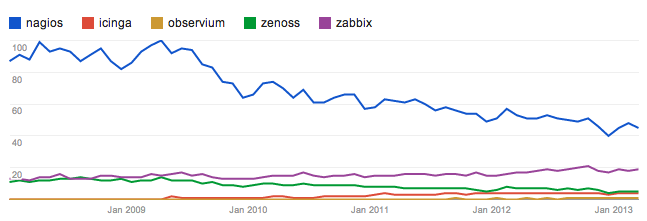
\includegraphics[scale=0.6]{img/monitoring_google_trends}
    \caption{Google Trends: overvåkningsløsninger}
    \label{losninger}
\end{figure}

\section{Valg av kjerneprogramvare}
Valg av kjerneprogramvare var gruppens viktigste valg, da det la grunnmuren for resten av prosjektet, og ville få stor innvirkning på sluttresultatet. Av kandidatene nevnt i \ref{sec:hvilkefinnes}, ble Icinga og Nagios videre vurdert.  

Icingas distribuerte system består av kjernen, som står for prossessering, et databaselag, og administrering av systemet via et webgrensesnitt. Dette er tilrettelagt for et distribuert oppsett. Nagios sin arkitektur har avhengigheter mellom web og lagring av status, som fører til at disse ikke kan separeres. Det er derimot mulig å separere ut MySQL-databasen som Nagios benytter\cite{icingaarchitecture}.

For uthenting av informasjon i Icinga er det utviklet et API som brukes via Icinga Web. Dette gir ett punkt for uthenting av data, med samme oppbygging for alle spørringer. I Nagios er det ikke noen standardisert måte å hente ut informasjon\cite{icingaapi}.

En annen fordel med Icinga er støtte for LDAP-autentisering i Icinga Web, som videre kan benyttes til å styre tilgang til ulik informasjon for brukere. Med Nagios kan en også innføre LDAP-støtte, men dette blir da autentisering via en web-server, og videre kontroll av aksess er ikke mulig. Nagios har noe aksesstyring, men det er bare på et objekt kalt ``contactgroups''. Icinga har aksesstyring på en rekke flere objekter\cite{icingaweb}.

For databaseoppsett støtter Icinga de tre databasemotorene PostgreSQL, Oracle og MySQL. Nagios har bare støtte for MySQL. I oppgavebeskrivelsen er det krav om MySQL, men for fremtidig bruk av Icinga er det mulighet for å benytte de to andre.

Icinga har også en tilleggsmodul kalt ``Icinga Mobile''. Denne gir tilrettelagt grensesnitt for mobile enheter, som var ønsket i oppgavebeskrivelsen. Icinga Mobile kan brukes for å gi et grensesnitt tilpasset mindre skjermer. Ved utsendelse av SMS eller e-post til en eller flere ansatte, kan Icinga-Mobile brukes via samme enhet for å se mer utfyllende informasjon om problemet, samt gjøre administrative handlinger.

Etter en vurdering av denne funksjonaliteten, ble det besluttet å basere overvåkningsløsningen på Icinga framfor Nagios.
\clearpage
\section{Icinga}
For å kunne forstå implementasjonsdelen av prosjektrapporten er det behov for noe innsikt i hvordan Icinga fungerer. I dette delkapittelet er det viktigste forklart.
\subsubsection{Arkitektur}
Icinga består av tre separate komponenter, som vist i Figur \ref{icingacomponents}.

\begin{figure}[H]
    \centering
    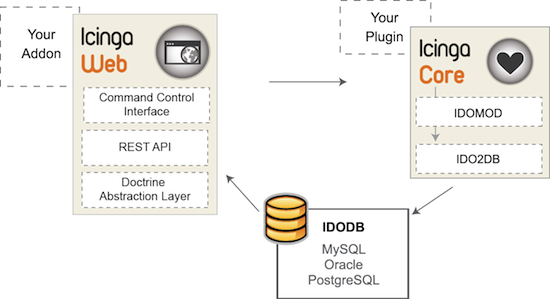
\includegraphics[scale=1.2]{img/icinga_architecture}
    \caption{Icingas tre komponenter}
    \label{icingacomponents}
\end{figure}

\subsubsection{Core}
Icinga Core håndterer planlegging av sjekker gjennom plugin-er og tar i mot resultatene av disse. Denne informasjonen sendes gjennom SSL-krypterte TCP-sockets videre til IDO2DB-prosessen (Icinga Data Out to Database) gjennom et interface kalt IDOMOD (Icinga Data Out Module). Ved å bruke disse abstraksjonslagene kan databasemotoren enkelt byttes ut. I dokumentasjonen er det laget veiledninger for MySQL, PostgreSQL og Oracle\cite{icingaarchitecture}.

IDOMOD og IDO2DB kommer i en samlet pakke (IDOutils), men kan separeres ut for å skape et distribuert oppsett. CERN i Sveits har nylig implementert et slikt oppsett med hjelp av lastbalansereren ``Mod Gearman''\cite{cernthesis}.

\subsubsection{Web}\label{sec:teoriweb}
I utgangspunktet kommer ikke Icinga med noe webgrensesnitt. Men det er mulig å installere to forskjellige pakker for å få dette. I begge kan en få en oversikt over tilstanden til enheter og tjenester, se konfigurasjon og utsendte varsler, samt utføre administrative oppgaver. Det kan også hentes ut statistikk over oppe- og nedetid.

Icinga Classic baserer seg på det samme vindusoppsettet som Nagios. For uthenting av data benyttes CGI-moduler som henter ut data fra filen ''status.dat''. Filen blir brukt av Icinga for å lagre tilstandsinformasjon om enheter og tjenester, kommentarer, og informasjon om nedetid. 

Icinga Web er en total omskrivning av webgrensesnittet. Det er en Ajax-drevet, Web 2.0-inspirert front-end, som har flere lag mellom kjernen av Icinga og visningene:

\textbf{Doctrine Abstraction Layer} henter informasjon fra databasen. Det kan også benyttes av utviklere for å legge til egne moduler i Icinga Web med uthenting av informasjon fra andre databaser.
\textbf{REST API} presenterer dataene fra DAL til Icinga Web. Her kan autentisering utføres slik at en kan sette hvilken informasjon ulike brukere skal kunne se.
\textbf{Command Control Interface} kan videresende kommandoer til Icinga Core. For eksempel manuell kjøring av en sjekk eller restart av Icinga. 

\section{Objekter}\label{sec:objekter}
All konfigurasjon av Icinga gjøres i tekstfiler. I selve konfigurasjonsfilen ''icinga.cfg'' settes filbanen til konfigurasjonsfilene. Icinga vil da ved oppstart lete rekursivt gjennom mappen etter filer som ender med ''.cfg''.

Konfigurasjonsdataene er bygget rundt det som i Icinga kalles objekter. Dette er en samling av konfigurasjon som hører sammen. Selv om en ikke kan si at Icingas objekter er det samme som objekter i programmeringsverden, benyttes mange av de samme begrepene og konseptene.

En rekke objekter er definert i Icinga, som vist i Tabell \ref{objekter}.

\begin{changemargin}{-1cm}{-1cm}
\begin{table}
\begin{center}
%\begin{tabular}{|p{2.0in}|c|c|c|} \hline
\begin{tabular}{ | p{3.5cm} | p{6.5cm} | p{6cm} |} \hline
	\textbf{Objekt} & \textbf{Forklaring} & \textbf{Eksempel} \\ \hline
	Host & En enhet med en adresse (typisk IP-adresse eller MAC-adresse). & Server, switch, router etc. \\ \hline
	Command & En kommando som skal kjøres på overvåkningsserveren & Et program, for eksempel check\_ping. \\ \hline 
	Service & Kombinasjonen av et host-objekt og et command-ojekt. & Sjekk oppetid: kommandoen ``check\_uptime'' skal kjøres på ``dc1''. \\ \hline
	Servicegroup & Service-objekt knyttet til host-objekter satt sammen til en applikasjon. & En applikasjon har tre prosesser som må være kjørende for at applikasjonen fungerer. Disse grupperes under samme servicegroup. \\ \hline
	Contact & Når og hvordan en person skal kontaktes angående en service. & Jens skal få en SMS hvis DHCP ikke er tilgjengelig. \\ \hline
	Timeperiod & Navn og definisjon av en tidsperiode. & Mellom 08.00 og 16.00 på annenhver tirsdag, hvis det er den tredje dagen i måneden. \\ \hline
	Host dependency & En eller flere avhengigheter. Dersom et host-objekt er avhengig av et annet, og det ikke svarer lenger, trenger ikke Icinga utføre sjekker på det avhengige objektet. & kantswitch1 er avhengig av kjerneswitch. \\ \hline
	Service dependency & Samme som host, men for service. & Captive portal er avhengig av RADIUS. \\ \hline
	Host escalation & Hva skal skje etter at en host har vært nede etter en definert tid. &	Om dc1 har vært nede i 30 minutter, send e-post til Ola Sysadmin. Etter 60 minutter sendes SMS til alle i admin contactgroup-en \\ \hline
	Service escalation & Samme som for objektet host-dependency, men for service-objeker. & Om DNS har vært nede i 30 minutter, send e-post til Kari Sysadmin. Etter 60 minutter send SMS til alle i admin hostgroup-en. \\ \hline
	\end{tabular}
	\caption{Oversikt over objekter i Icinga}
	\label{objekter}
\end{center}
\end{table}
\end{changemargin}

I tillegg til disse kan host, service og contact grupperes med henholdsvis hostgroup, servicegroup og contactgroup.

Det er også to objekter med metainformasjon, ``hostextinfo'' og ``serviceextinfo'', der en kan definere ekstra konfigurasjon som bildebaner, notater og koordinater for host- og service-objekter.

Den siste objekttypen er module. Her spesifiseres konfigurasjon for en modul som utvider funksjonalitet i Icinga Web.

Sammenhengen mellom objektene er viktig å forstå for å skjønne hvordan sjekker utføres i Icinga. I et service-objekt defineres hvilket command-objekt som skal benyttes for å teste tjenesten og hvilke host- eller hostgroup-objekter dette skal sjekkes på. Dette er vist i Figur \ref{command_host_service}.

\begin{figure}[H]
    \centering
    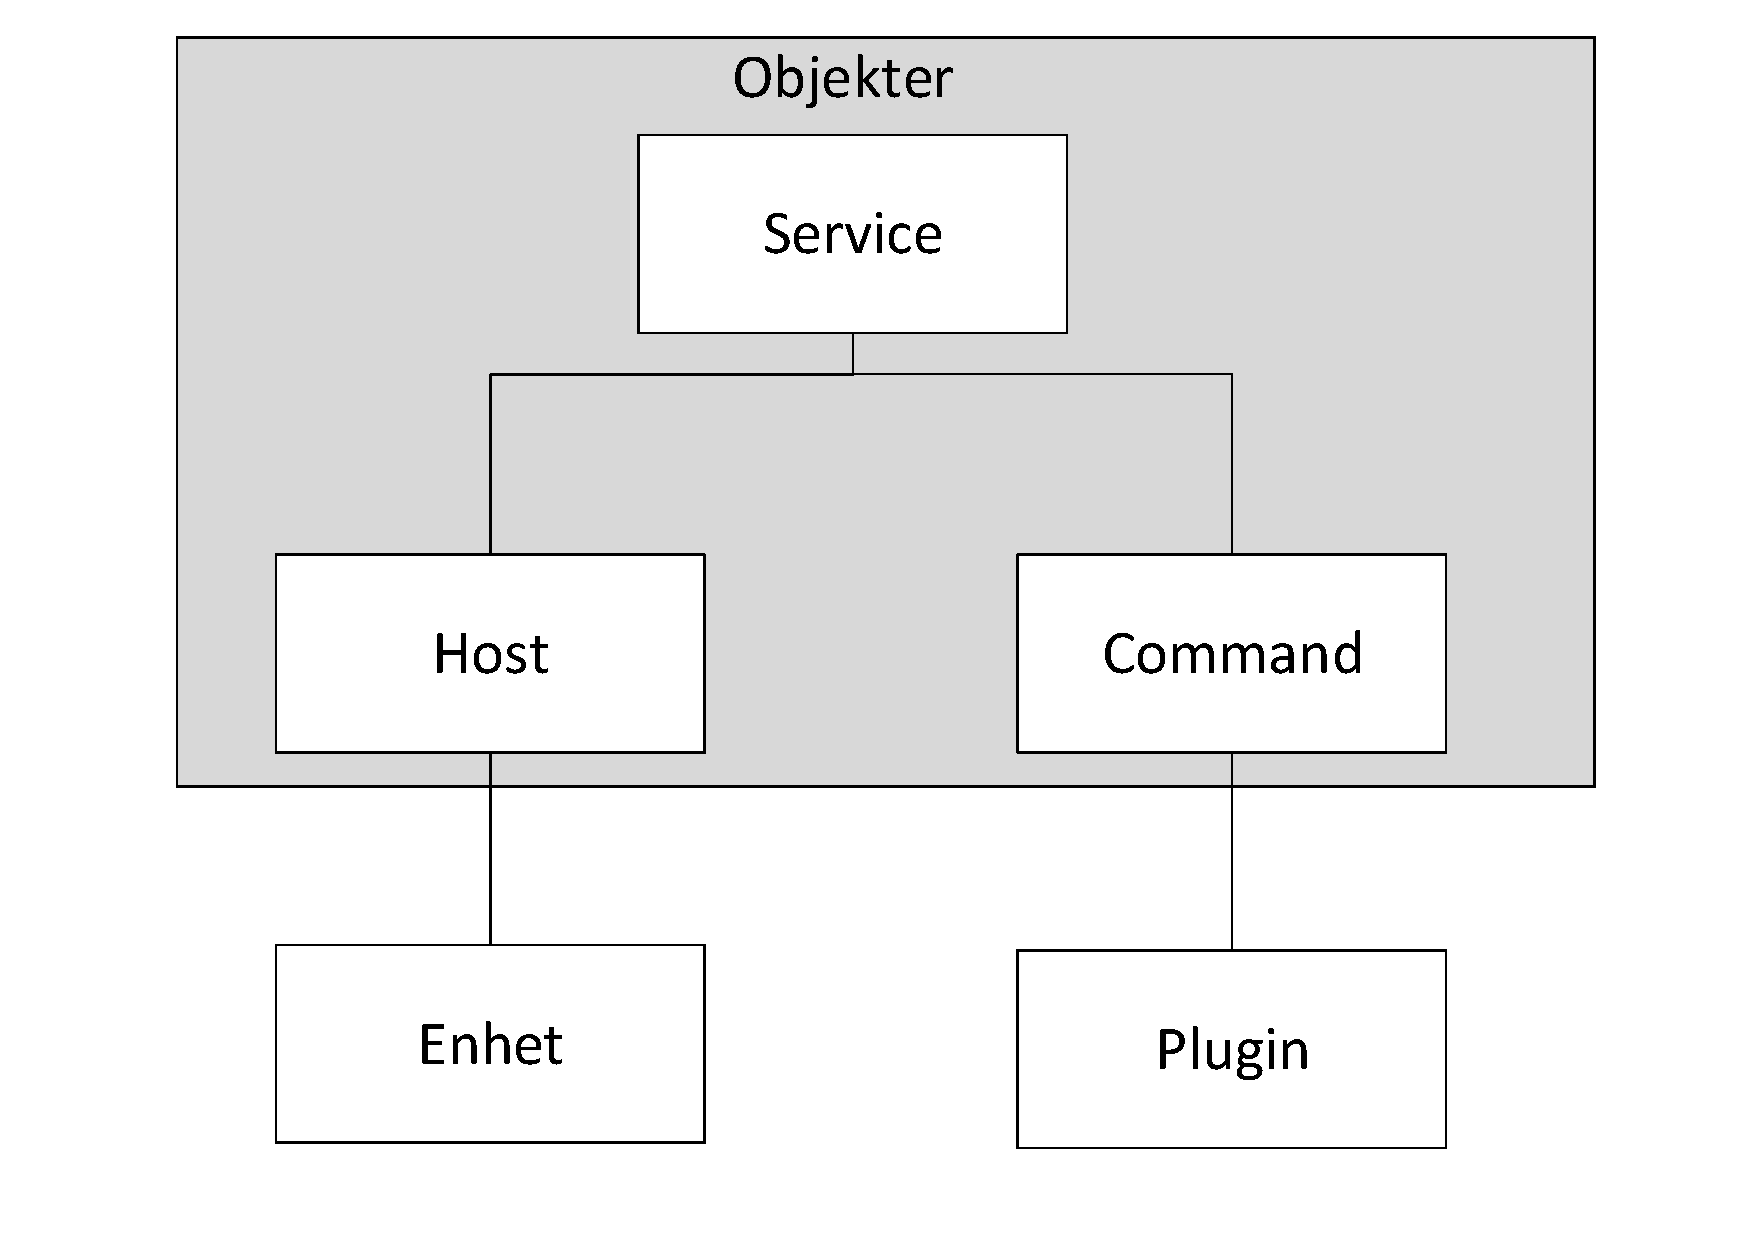
\includegraphics[scale=0.4]{img/command_host_service}
    \caption{Sammenhengen mellom host-, service- og command-objekter.}
    \label{command_host_service}
\end{figure}
% Si noe om utelatt konfig, arv ved use?
I eksempelet under vises konfigurasjonen for å sette opp en ping-sjekk på HiG1.
\begin{lstlisting} [style=example]
define host {
    use                  generic_host
    host_name            HiG1
    address              192.168.0.1
}

define service {
    use	                 generic_service
    host_name            HiG1
    service_description  Ping
    check_command        check_ping!200,5%!500,10%
    check_interval       5
}

define command {
    command_name         check_ping
    command_line         /usr/lib/nagios/plugins/check_ping -H $HOSTADDRESS$ --warning $ARG1$ --critical $ARG2$   
}
\end{lstlisting}

\clearpage
\section{Plugin-er}
Icinga i seg selv kommer uten noen overvåkningssjekker. Til dette benyttes plugin-er.

En plugin i Icinga er et eksternt program som kjøres og outputen hentes inn som data. Resultatet av sjekken hentes fra exit-koden\cite{wiki:returncode} og oversettes til en tilstand, som vist i Tabell \ref{state}.

En plugin kan være noe helt enkelt som scriptet under. Der exit-koden til en ping-kommando sjekkes. Hvis ping ikke får svar, vil den gi exit-koden 1. Scriptet vil da gi exit koden 2, som i Icinga oversettes til CRITICAL.
\begin{lstlisting}[language=bash]
#!/usr/bin/env bash
loss=$(ping -c 5 google.com)
if [ $? -eq 0 ]; then
    echo "OK"
    exit 0
else
    echo "ERROR"
    exit 2
fi
\end{lstlisting}

Det finnes et sett med offisielle plugin-er til Nagios; nagios-plugins, som utgis av ``Nagios Plugins project''. Pakken finnes i en rekke pakkebehandlere og inneholder over 50 plugin-er som er ment for å dekke et grunnleggende overvåkningsbehov\cite{nagiosplugins}.

\begin{table}[H]
	\begin{center}
	\begin{threeparttable}
	\begin{tabular}{| l | l | l |} \hline
	\textbf{Returkode fra plugin} & \textbf{Service-tilstand} & \textbf{Host-tilstand} \\ \hline
	0 & OK & UP \\ \hline
	1 & WARNING & UP eller DOWN/UNREACHABLE* \\ \hline
	2 & CRITICAL & DOWN/UNREACHABLE \\ \hline
	3 & UNKNOWN & DOWN/UNREACHABLE \\ \hline
	\end{tabular}
	\begin{tablenotes}
	\small
	\item *Ved bruk av Aggressive host checking\cite{icingapluginapi}.
	\end{tablenotes}
	\caption{Tilstandsoversikt}
	\label{state}
	\end{threeparttable}
	\end{center}
\end{table}

\section{Sjekker}\label{sec:sjekker}
Tilstanden for et service- eller host-objekt vil bestemmes ut i fra et returnert resultat fra en aktiv eller passiv sjekk. Forskjellen på disse to vil bli forklart i de neste delkapitlene.

Dersom en aktiv eller passiv sjekk resulterer i en annen tilstand enn OK, er det to typer av tilstanden, ``SOFT'' og ``HARD''. Første gang en plugin returnerer en feil vil tilstanden bli satt til SOFT, i tillegg til service- eller host-tilstanden. Etter dette vil sjekken kjøres hyppigere for å finne ut om det er snakk om et forbigående problem. Etter et gitt antall ganger der plugin-en fortsatt ikke returnerer OK, vil tilstanden skifte til HARD og det sendes ut varslingsmelding. Varsling er beskrevet grundigere i \ref{sec:varsling}.

\clearpage
\subsubsection{Aktive sjekker}
En aktiv sjekk er en sjekk som initieres av Icinga, der en kommando kjøres på Icinga-serveren. Dette er også kjent som en ``poll''-modell. En aktiv sjekk defineres ut i fra et command-objekt med parametere og et tidsintervall i service- og host-objekter. I command-objektet defineres en plugin som skal kjøre, og returverdien fra denne vil bestemme hvilken tilstand service- eller host-objektet har. I Figur \ref{active_checks} vises komponentene involvert i en aktiv sjekk.
\begin{figure}
   \centering 
   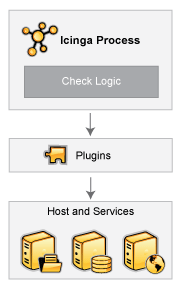
\includegraphics[scale=0.7]{img/activechecks.png}
    \caption{Aktive Sjekker}
    \label{active_checks}
\end{figure}

\subsubsection{Passive sjekker}
Passive sjekker går motsatt vei av aktive sjekker. Her vil hver host si ifra når verdier har overgått en satt grense eller en feil har oppstått. Dette kalles ofte for en ``push''-modell. Passive sjekker kjøres ved at et eksternt program skriver en linje med informasjon om tjenesten og sjekkresultat til en fil, som Icinga sjekker periodisk. Dette er illustrert i Figur \ref{passive_checks}.

Fordelen med passive sjekker er at Icinga vil oppdage feil raskere. Ved standard konfigurasjon sjekkes filen med sjekkresultater så ofte som mulig, mens aktive sjekker kjøres hver 5. minutt. Passive sjekker vil også avlaste Icinga-serveren, da alle sjekker utelukkende vil bli kjørt lokalt på enheten som overvåkes. Men en må åpne for at kommunikasjon kan initieres fra alle enheter som skal overvåkes til Icinga-serveren, og mister da samtidig muligheten til å samle all konfigurasjon på ett sentralt sted. 

\begin{figure}[H]
    \centering
    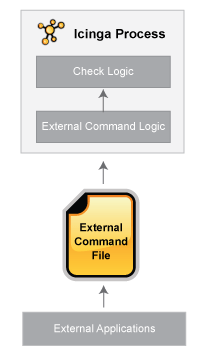
\includegraphics[scale=0.7]{img/passivechecks.png}
    \caption{Passive Sjekker}
    \label{passive_checks}
\end{figure}

\subsubsection{Hostsjekk}
Resultatet av en host-sjekk vil avgjøre om tilstanden til host-objektet er ``UP'' eller ``DOWN''. 

Det er ikke et fast tidsintervall for en hostsjekk med mindre check\_interval er definert for objektet. Icinga vil kjøre sjekken om en service som er satt opp for host-en skifter tilstand. Service-objekter som er definert for en host som er i ``DOWN'' vil automatisk bli vist under ``Known service problems'' i webgrensesnittet, og ingen sjekker vil bli kjørt på dem før host-en er ``OK'' igjen.

Grunnsjekken for en host defineres i host-konfigurasjonen med ''check\_command'', som vist under.
\begin{lstlisting}[style=example]
define host {
...
    check_command	check_host_alive
}
\end{lstlisting}

\subsubsection{Variabler}
For å kunne gjøre konfigurasjon av Icinga mest mulig dynamisk er det en rekke forhåndsdefinerte variabler en kan bruke i konfigurasjonsfilene. Disse kalles makroer. En fullstendig liste over disse og hvor de kan benyttes finnes i Icinga-dokumentasjonen\cite{icingamacro}. ''\$HOSTADDRESS\$'' kan for eksempel benyttes i et command-objekt slik at det bare må skrives en gang, og ikke for hver host. En kan også definere egne variabler som for eksempel ''\_SSHPORT''. Disse kan sendes videre til selve kommandoen som kjøres og benyttes som argumenter til plugin-en som kjører en sjekk, slik:
\begin{lstlisting}[style=example]
define host {
...
    host_name		example_server
    _SSHPORT		222
}
define command {
    command_name	check_ssh
    command_line	$USER1$/check_ssh -H $HOSTADDRESS$ -p $_HOSTSSHPORT$
}
\end{lstlisting}

Her benyttes de innebygde variablene ``USER1'' for banen til plugin-en som kjøres, HOSTADDRESS for IP-en til den hosten som sjekken skal kjøres på og den egendefinerte variabelen \_SSHPORT som defineres på host-objektet.

USER-variablene defineres i den globale konfigurasjonsfilen og brukes der hvor informasjon skal sjules fra webgrensesnittet. Som for eksempel når det trengs et passord for å utføre en sjekk.

\subsubsection{Templates}
En template er ikke et objekt i seg selv, men en mal for et objekt. Med direktivet ``register 0'' vil ikke Icinga registrere dette objektet for overvåkning. Ved å bruke direktivet ``use'' kan en i et annet objekt ``arve'' konfigurasjonen fra template-en. Template-er kan også arve, og en kan dermed sette opp et hierarki der en spesifiserer generell konfigurasjon i toppen og arver nedover til mer spesiell. 

I eksempelet under er generell konfigurasjon for alle host-objekter definert i ``generic\_host'', som brukes i de andre objektene. I ``generic\_firewall'' erstattes verdien for kontaktgruppe, og i cisco\_firewall settes en egendefinert variabel:

Template-en generic\_host: 
\begin{lstlisting}[style=example]
define host {
    name                            generic_host    ; The name of this host template
    notifications_enabled           1       ; Host notifications are enabled
    event_handler_enabled           1       ; Host event handler is enabled
    flap_detection_enabled          1       ; Flap detection is enabled
    failure_prediction_enabled      1       ; Failure prediction is enabled
    process_perf_data               1       ; Process performance data
    retain_status_information       1       ; Keep status after Icinga restart
    retain_nonstatus_information    1       ; Keep non-status after Icinga restart
    check_command                   check-host-alive
    max_check_attempts              10
    normal_check_interval           5
    retry_check_interval            2
    notification_interval           0
    notification_period             24x7
    notification_options            d,u,r
    contact_groups                  all_contacts
    register                        0       ; Not a real host, just a template
}
\end{lstlisting}

Template-en generic\_firewall, som arver fra generic\_host:
\begin{lstlisting}[style=example]
define host {
   name             generic_firewall
   use              generic_host
   contact_groups   firewall_admins
   register         0
}
\end{lstlisting}

Template-en cisco\_firewall, som arver fra generic\_firewall:
\begin{lstlisting}[style=example]
define host {
    name            cisco_firewall
    use             generic_firewall
    register        0
    _WANPORT        WAN ; Custom variable for WAN port to monitor
}
\end{lstlisting}

Host-objektet hig-hw1, som arver fra cisco\_firewall:
\begin{lstlisting}[style=example]
define host {
    use             cisco_firewall
    host_name	    hig-fw1
}
\end{lstlisting}

Dette gjør at det blir lite konfigurasjon hver gang en ny brannmur skal legges til.

\subsubsection{Regulære uttrykk}
Ved å sette ``use regular expressions'' i konfigurasjonen for Icinga, kan en benytte regulære uttrykk i attributter i et objekt, der en refererer til andre objekter. Icinga støtter standarden POSIX Extended Regular Expressions, og vil automatisk tolke navnet på objekter som et regulært uttrykk dersom det inneholder \verb|"*", "?", "+", eller "\"|.

Dette kan være nyttig dersom en for eksempel vil legge alle hoster i en hostgroup, som har en navnekonvensjon som gjør at hver av hostene unikt kan identifiseres ved å bytte ut deler av navnet med en variabel.

I eksempelet nedenfor brukes det regulære uttrykket \verb|"^HiG\[0-9\]+\$"| i attributten ``members'' til å legge til alle konfigurerte hosts der navnet starter på ``HiG'' etterfulgt og avsluttet med ett eller flere siffer mellom 0 og 9, i hostgroup-objektet ``all\_servers''.
\begin{lstlisting}[style=example]
define hostgroup {
    hostgroup_name	all_servers
    alias		All Servers
    members		^HiG[0-9]+$
}
\end{lstlisting}

Det kan også benyttes til å ekskludere en host fra en service-sjekk. I eksempelet nedenfor er HiG3 medlem av hostgroup-en ``windows\_servers'', men blir ekskludert fra å kjøre sjekken på diskplass ved å sette ``!HiG3'':
\begin{lstlisting}[style=example]
define service {
    use				generic_service
    service_description		Disk space
    hostgroup_name		windows_servers
    host_name			!HiG3
    check_command		win_nrpe!CheckDriveSize!Drive="C" MaxWarnUsed=80% MaxCritUsed=90%
}
\end{lstlisting}

\section{Avhengigheter}
I Icinga kan en definere tre ulike typer avhengigheter, ``Parent'', ``Service dependency'', og ``Host dependency''. Disse har innvirkning på hvilke varsler som sendes ut og statusen de ulike service- og host-objektene får. Hver av disse krever egen konfigurasjon. 

\section{Parent}\label{sec:parent}
Et host-objekt kan settes som en parent til et annet host-objekt. Host-objekter som har en parent blir betegnet som en child-host eller child-service. Dette brukes primært for å unngå varsler om andre host- og service-objekter enn det som er definert som parent, om denne blir utilgjengelig. For eksempel hvis kjernerouteren mister strømtilgangen, ønskes ikke varsler for eventuelle host-objekter og tilhørende service-objekter som har kjernerouteren som parent. Disse vil ikke lenger bli sjekket og tilstanden vil bli satt til ``UNREACHABLE''. Tjenester som tilhører host-ene vil få tilstanden ``UNKNOWN''.

For redundante oppsett kan et host-objekt ha flere ``parents'' definert. Host-objektet vil da ha tilstanden UP så lenge minst én ``parent''-host er UP.

Ut ifra parent-relasjonene mellom host-objekter i konfigurasjonsfilene genereres også et ``Status Map'' over nettverket, som vist i Figur \ref{statusmap}. Dette brukes til å visualisere alle relasjonene, og vil gjengi redundante oppsett og hvilke host-objekter som er påvirket av at parent-hosten er DOWN.

\begin{figure}[H]
    \centering
    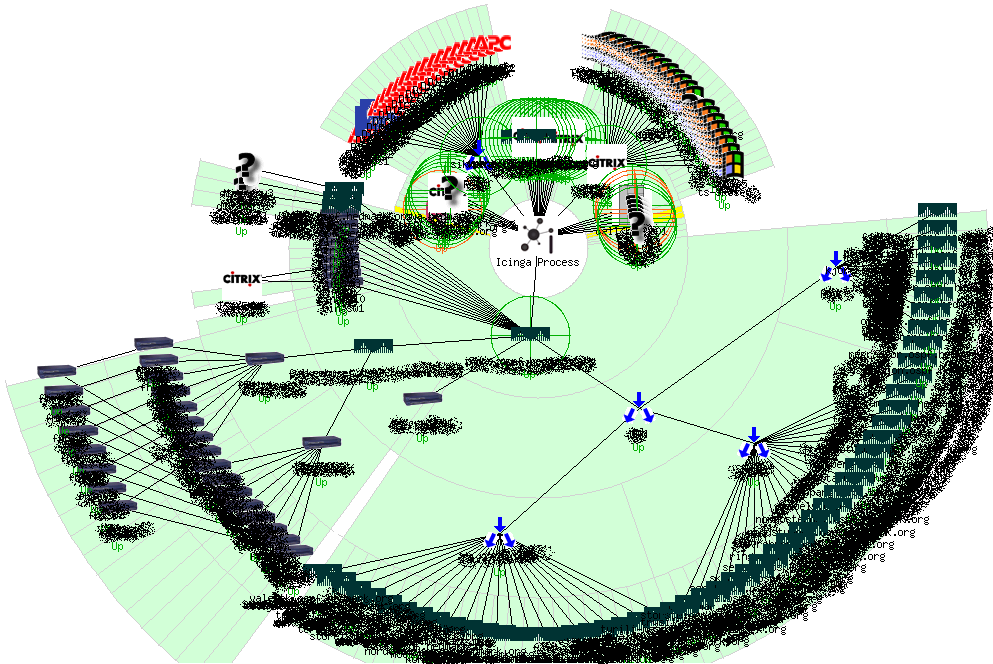
\includegraphics[scale=0.6]{img/statusmap}
    \caption{Kart som viser parent- og host-relasjoner}
    \label{statusmap}
\end{figure}

\section{Service dependency}\label{sec:servicedependency}
Service dependency er en egen objekttype der en kan sette opp avhengighet mellom to service-objekter. Formålet med dette er å unngå varsel hvis en tjeneste får tilstanden DOWN, som følge av at en annen tjeneste har det. For eksempel bør det ikke varsles om at tjenester som er avhengig av autentisering via LDAP-serveren får ``Access Denied''-feilmeldinger, hvis LDAP-serveren er DOWN. Det service-objektet andre service-objekter er avhengige av kalles en master service. 

Icinga undersøker om avhengigheter er definert for et service-objekt, før det utføres sjekker på det. Dette er med på å bestemme om det blir sendt ut varsel for service-objektet.

I eksempelet under er tjenesten ``Check SMB'' på HiG3 avhengig av master-service-en Check LDAP på HiG3. ``execution\_failure\_criteria'' bestemmer ved hvilke tilfeller tjenesten ikke skal sjekkes. Her er den satt til ``c'', som vil si at Check SMB ikke skal kjøres dersom ``Check LDAP'' er i CRITICAL tilstand.

\begin{lstlisting}[style=example]
define servicedependency {
    host_name                          HiG3
    service_description                Check LDAP
    dependent_host_name                HiG3
    dependent_service_description      Check SMB
    execution_failure_criteria         c
    notification_failure_criteria      c
}
\end{lstlisting}

Ved standard konfigurasjon vil Icinga benytte siste harde tilstand for master service. Dersom ``max\_check\_attempts'' for eksempel er satt til 4, vil ikke Check SMB stoppes fra å kjøres før Check LDAP har blitt sjekket fire ganger, og oppnår en hard tilstand. 

På attributten notification\_failure\_criteria kan det settes hvilke service-tilstander en ikke skal varsle for. Dette er hovedgrunnen til at det settes opp slike avhengigheter. Når denne er satt til ``c'' vil det ikke varsles om master service-en får tilstanded CRITICAL.

Service-objekter har kan også arve avhengighetene til en master service ved å sette direktivet ``inherits\_parent 1''. For eksempelet over vil Check SMB da arve fra service-objekter som Check LDAP arver fra.

For å konfigurere avhengigheter mellom tjenester som kjører på samme host kan en utelate ``dependent\_host\_name'' I eksempelet under vil alle tjenester på host-objektet være avhengig av tjenesten ``NRPE-daemon''.

\begin{lstlisting}[style=example]
define servicedependency{
    ;dependent_host_name   	    ; Not defined to make dependancy on same host            
    hostgroup_name 		    linux_servers
    service_description             NRPE-daemon
    dependent_service_description   NRPE Check *
    execution_failure_criteria      c
    notification_failure_criteria   c
}
\end{lstlisting}

En kan også erstatte host\_name og dependant\_host\_name med hostgroup og dependant\_host\_group for å lage avhengigheter på alle objekter som tilhører gruppen.

\section{Host dependency}
For å sette en avhengighet mellom to host-objekter benyttes host dependency. Dette må ikke forveksles med parent, som refererer til nettverksoppsettet. En host dependency vil si at et host-objekt er avhengig av et annet host-objekt. Host dependency er bare nyttig i veldig spesielle tilfeller, da det for de fleste tilfeller vil være avhengigheter til en eller flere tjenester på host-en\cite{hostandservicedep}, eller at en host er avhengig av å kjøre en sjekk igjennom en annen host.

\section{Protokoller og agenter}
For å kjøre sjekker på enheter må Icinga-serveren kunne kommunisere med operativsystemene på de ulike enhetene. Icinga henviser til protokollene SSH, SNMP, RPC (WMI) og agentene NRPE og NSCA (en del av pakken NSClient++) i dokumentasjonen\cite{icingaintegration,icingaadditionalsoftware}. 

\subsubsection{NRPE}\label{sec:nrpe}
NRPE (Nagios Remote Plugin Executor) består av plugin-en ``check\_nrpe'' på Icinga-serveren og en daemon som installeres på hver server som skal overvåkes. NRPE eksekverer lokale plugin-er på den eksterne serveren og returner dataen fra denne til check\_nrpe. Tillatelse for eksekveringer defineres i en konfigurasjonsfil på hver server, der en oppgir hvilke IP-adresser som kan koble seg til og hvilke kommandoer som er gyldige. 

\begin{figure}[H]
    \centering
    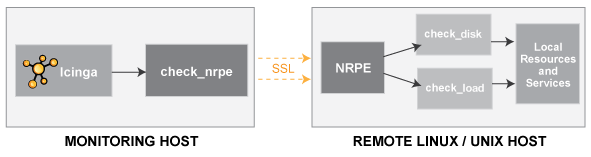
\includegraphics[scale=0.6]{img/nrpe.png}
    \caption{NRPE}
    \label{nrpe}
\end{figure}

\subsubsection{SSH}
Gjennom en tilkobling til en SSH (Secure Shell)-server kan en spesifisere en kommando som skal kjøres på en ekstern maskin, og hente output-en til det opprinnelige shellet. Dette virket som den beste måten å overvåke Linux-servere på, ved starten av prosjektet. SSH-prosjektet er meget utbredt og blir aktivt sjekket for sikkerhetshull. SSH er også installert på de aller fleste Linux-servere, og en vil dermed unngå å lytte på en ekstra port.

Ulempen med å kjøre sjekker over SSH er at en må sette opp nøkkelbasert innlogging mellom Icinga-serveren og alle Linux-serverne som skal overvåkes. En kan begrense rettigheter for brukeren som kjører sjekkene, men den vil fortsatt ha muligheten til å logge inn til et shell og eksekvere kommandoer. Dette kan føre til at en potensiell angriper via Icinga-serveren, har en vei inn til alle servere som overvåkes, ved å bruke den private nøkkelen.

SSH gir også endel overhead både på nettverkstrafikk og i CPU-tid\cite{sshmanpage}. En måte å begrense dette på er å benytte SSH med ControlMaster. Dette innebærer en endring i SSH-konfigurasjonen på serveren, slik at SSH-klienten lagrer informasjon om hver utgående TCP-tilkobling, og samme tilkobling kan benyttes mot samme host. Dermed unngås en ny TCP-tilkobling for hver ny sjekk som skal utføres på hosten.

\subsubsection{SNMP}
Det meste av nettverksutstyr beregnet for bedrifter, har i dag støtte for protokollen SNMP (Simple Network Management Protocol\cite{essentialsnmp}). SNMP definerer en enkel og effektiv måte å overvåke enheter på og det gir en standard som leverandørene følger.
	
SNMP baserer seg på variabler som blir gjort tilgjengelig på enheten som skal overvåkes (kalt agenten). Disse variablene er definert i en Management Information Base (MIB). MIB-filene er ofte tilgjengelige på produsentens hjemmeside. Her beskrives strukturen for dataen i et hierarkisk navnerom som inneholder Object Identifier (OID). Hver OID identifiserer en variabel som kan bli lest eller satt via SNMP. Enheten som ber om disse variablene kalles ``manager''. 

En ulempe med SNMP er at OID-ene er lange og tunge å lese. For eksempel for å hente ut batterikapasiteten på en APC UPS benyttes OID-en:
\
1.3.6.1.4.1.318.1.1.1.2.2.1.0
\
Dette kan oversettes til:
\
iso(1). org(3). dod(6). internet(1). private(4). enterprises(1). apc(318). products(1). hardware(1). ups(1). upsBattery(2). upsAdvBattery(2) upsAdvBatteryCapacity.0
\
Denne OID-en er definert i APCs MIB-fil ``PowerNet MIB''. Ved å laste inn denne kan en også benytte ``PowerNet-MIB::upsAdvBatteryCapacity.0''.

SNMP finnes i flere versjoner. I dag brukes for det meste versjon 2c og den nyeste, versjon 3. De ulike versjonene er ikke kompatible, men i praksis støtter det meste av utstyr som støtter v3 eller v2c også v1 \cite{rfc3584}. Hovedforskjellen på versjon 2c og 3 er at versjon 3 har støtte for flere sikkerhetsmekanismer, men krever noe mer konfigurasjon. Sikkerhetsaspektet ved dette er diskutert videre i Kapittel \ref{chap:sikkerhet}.

Det eksisterer to muligheter når enheter skal overvåkes via SNMP. Enten kan enhetene selv rapportere inn hendelelser via SNMP trap/inform, eller så kan serveren spørre enhetene via SNMP GetRequest. Valg av det første medfører at en kan gjøre varsling umiddelbart, men da må også hver enhet konfigureres med parametere for hvilke trap-meldinger som skal sendes og til hvilken IP-adresse. Icinga har ingen støtte for å motta trap-er, men en kan installere en egen daemon for dette og rapportere inn data med passive sjekker. 

For å benytte SNMP trap/inform må en tillate tilkoblinger til overvåkingsserveren i stedet for bare fra denne. Hvilke trap-meldinger som skal sendes må også konfigureres på hver enhet, og en vil da ikke kunne ha alle konfigurasjoner sentralisert på Icinga-serveren.

\begin{figure}[H]
    \centering
    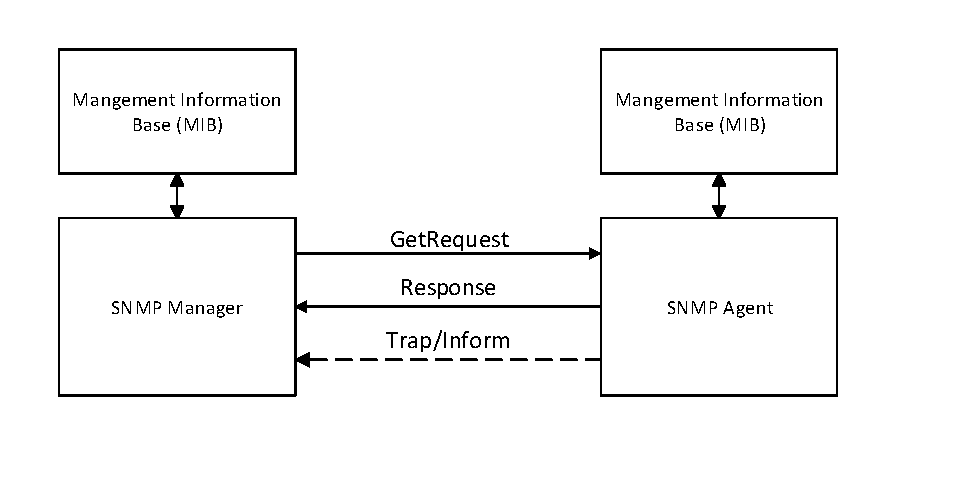
\includegraphics{img/SNMP}
    \caption{Overvåkning med SNMP}
    \label{SNMP}
\end{figure}

SNMP benytter seg av UDP for å levere trap-meldinger. UDP er en såkalt upålitelig protokoll, noe som vil si at det ikke er noen omsending av pakker eller noen tilbakemelding (ack) for at pakkene kommer fram. Derfor kan en risikere å miste en trap. SNMP inform, som kom i SNMPv3, løser dette ved at agenten vil sende en ny inform-pakke i et intervall, helt til manageren gir beskjed om at trap-meldingen er mottatt.

For å benytte SNMP på Windows- og Linux-servere kreves installasjon av en SNMP-agent\cite{mssnmp,netsnmp}.

\subsubsection{WMI (Windows Management Instrumentation)}
WMI er et grensesnitt som gjør det mulig å lage programmer eller script som utfører oppgaver mot operativsystemet Windows, både lokalt eller på eksterne maskiner. Disse oppgavene kan være alt fra å restarte maskinen, til å hente ut logger over hendelser som har inntruffet på maskinen. I en overvåkningsløsning vil det være mest relevant å kjøre kommandoer som henter ut informasjon om maskinen og tjenester som kjører på den. Dette kan for eksempel være hvilke prosesser som bruker mest CPU-tid.

For å benytte WMI-spørringer direkte fra en ekstern enhet må det konfigureres brukertilgang og brannmurregler\cite{wmiremote}. Med NSclient++ har en mulighet til å kjøre WMI-spørringer over NRPE uten ekstra konfigurasjon.

\subsubsection{Valg av Agenter}
Valg av protokoll eller agenter har basert seg på følgende punkter:
\begin{itemize*}
	\item Ressursbruk (CPU)
	\item Nettverkstrafikk
	\item Utrulling
	\item Sikkerhet
\end{itemize*}
Nettverkstrafikken som ble generert ved både en NRPE- og en SSH-sjekk ble målt ved å benytte et Bash-script som kjørte en disk-sjekk 100 ganger, som vist under. 

\begin{lstlisting}[style=example,language=bash]
#!/usr/bin/env bash
if [ "$1" == "ssh" ]; then
    cmd="/usr/lib/nagios/plugins/check_by_ssh -H 10.60.0.21 -C \"/usr/lib/nagios/plugins/check_disk -W 10% -C 5% -M -A\" > /dev/null"
elif [ "$1" == "nrpe" ]; then
    cmd="/usr/lib/nagios/plugins/check_nrpe -H 10.60.0.21 -c check_all_mounts -a 10,5 > /dev/null"
else
    echo "You must specify ssh or nrpe as the first argument"
    exit 1
fi
for i in {1..100}; do
    eval $cmd
done
exit 0
\end{lstlisting}

Både serveren og klienten stod i et eget nettverk i Virtualbox sammen med en Windows-maskin med et nettverkskort satt i promiscious mode, for å kunne sniffe nettverkstrafikken. Denne fanget nettverkstrafikken med Wireshark. Trafikken mellom de to maskinene ble hentet ut og data for hver tilkobling ble brukt til å kalkulere båndbreddebruk.

Det ble også undersøkt hvor mye CPU-tid NRPE og SSH trenger for å utføre sjekker. Fordi hver sjekk går veldig raskt ble det kjørt 100 disksjekker, 100 ganger. ``time''-kommandoen ble brukt for å se på tiden brukt i user- og kernel-mode. Dette ble gjort ved å bruke Bash-scriptet nedenfor, som kjører det samme scriptet som ble brukt for å generere nettverkstrafikk.

\begin{lstlisting}[style=example]
#!/usr/bin/env bash

args=(nrpe ssh)

for arg in "${args[@]}"; do
        for i in {1..100}; do
                /usr/bin/time -f "%U\t%S" run_check.sh $arg
        done
done
exit 0
\end{lstlisting}

\begin{figure}[H]
    \centering
    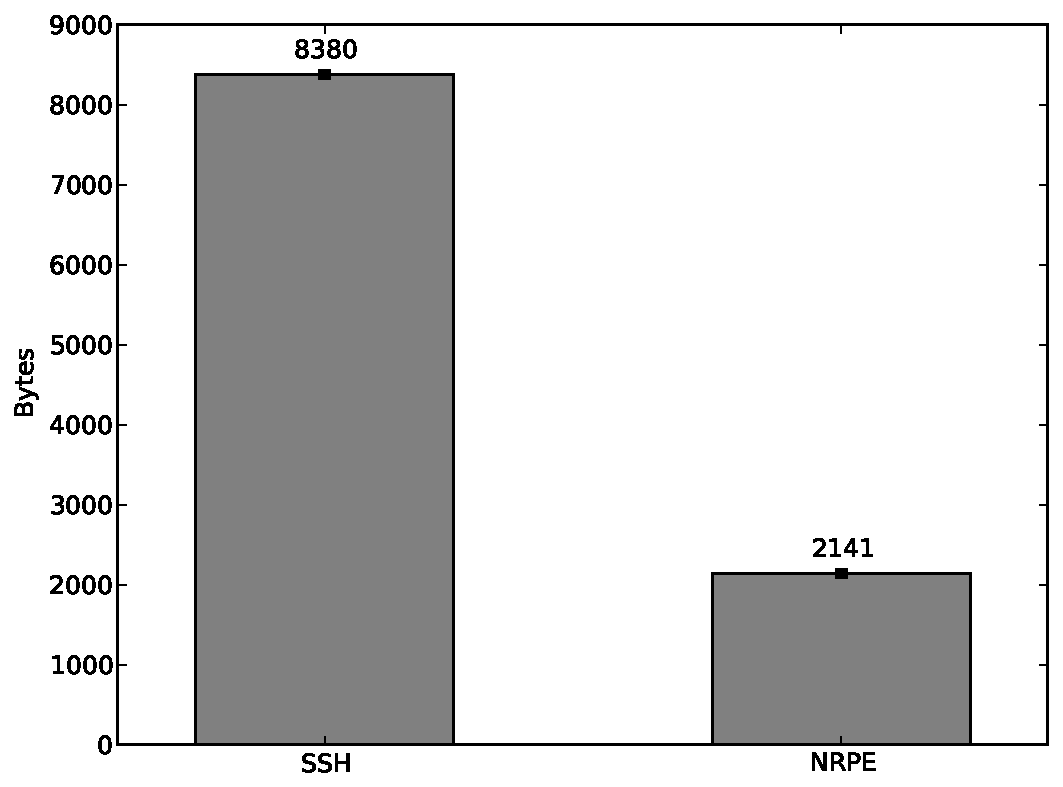
\includegraphics[scale=0.6]{img/nettverkstrafikk}
    \caption{Nettverkstrafikk}
    \label{network_traffic}
\end{figure}

\begin{figure}[H]
    \centering
    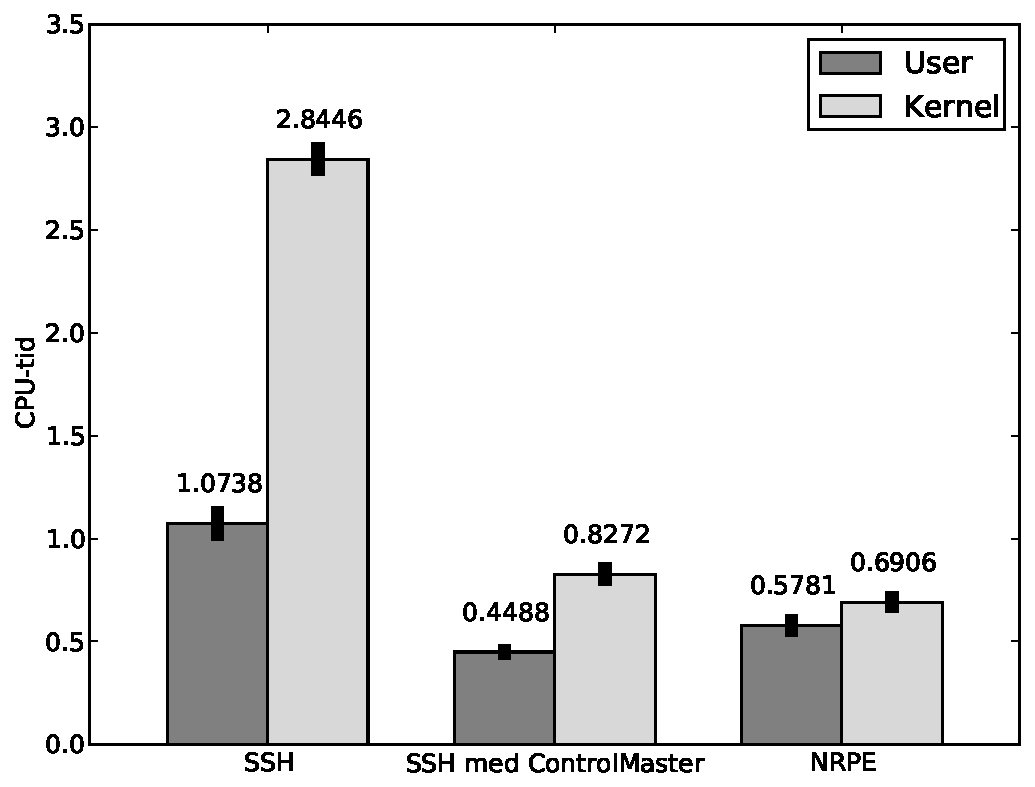
\includegraphics[scale=0.6]{img/cpubruk}
    \caption{CPU-bruk}
    \label{cpu_usage}
\end{figure}

\begin{table}
    \begin{center}
	\begin{threeparttable}
    \begin{tabular}{| l | l | l | l |} \hline
	\ & \textbf{CPU-tid i user(s)} & \textbf{CPU-tid i kernel(s)} & \textbf{Nettverkstrafikk (B)} \\ \hline
	SSH & 1.0738 (0.0792) & 2.8446 (0.0771) & 8380 (101.38) \\ \hline
	NRPE & 0.5781 (0.0347) & 0.6906 (0.0495) & 2141 (55.08) \\ \hline
	SSH med ControlMaster & 0.4488 (0.0509) & 0.8272 (0.0543) & 1700* \\ \hline
	\end{tabular}
	\begin{tablenotes}
	\small
	\item *For SSH med ControlMaster var det ikke mulig å separere ut hvor mye trafikk det var på én sjekk. Her er det brukt et gjennomsnitt ved å dele den totale mengden trafikk på antall sjekker.
	\end{tablenotes}
	\caption{Prosessorforbruk test med agenter}
	\label{agentcheck}
	\end{threeparttable}
	\end{center}
\end{table}
For en utrulling i den skalen som vil være aktuelt for IKT-avdelingen vil ikke denne nettverkstrafikken være noen stor faktor. Figur \ref{network_traffic} viser at gjennomsnittlig vil total båndbreddebruk for en sjekk var 8380 byte. Selv med 1000 enheter som overvåkes over SSH, der hver kjører 100 sjekker hvert 5. minutt, vil den totale båndbreddebruken, dersom alle sjekkene var jevnt fordelt over 5 minutters-intervallet:
\[\frac{8.38\:kB\times(1000\:(enheter)\times100\:(sjekker))\times8\:b/B}{5\:(min)\times60\:s}=22346.67\:Kb/s = 22.35\:Mb/s \] 
På et gigabit-nettverk, som i tillegg er full duplex, vil ikke dette være nevneverdig. Icinga vil forsøke å fordele sjekkene utover slik at lasten på Icinga-serveren og enhenetene som overvåkes blir minst mulig\cite{icingascheduling}, men i praksis blir ikke dette helt jevnt fordelt, tallet kan derfor bli noe høyere.

Resultatene av testen av CPU-tid i \ref{cpu_usage}, viser at SSH krever mer CPU-tid enn NRPE. Mye av dette er på grunn av overhead ved tilkobling og frakobling, som tallene for SSH med ControlMaster viser. 

Det ble valgt å benytte NRPE både for Linux- og Windows-servere. En fordel med dette er at samme protokoll for alle tilkoblinger fra Icinga-serveren til samme port (5666) på andre servere kan benyttes. Dette gjør at det kun trengs én brannmurregel for Icinga, som igjen holder antall angrepsvektorer nede. En annen fordel er at samme service- og command-objekter kan benyttes i Icinga for sjekker som skal utføres via NRPE, uavhengig av om hosten kjører Windows eller Linux.


%See page \pageref{status1.1} till \pageref{status2.1}.

\section{Implementering}
\subsection{Utstyr}
\subsubsection{Labmiljø}
Et labmiljø har vært brukt for å teste plugins og script før de blir implementert på produksjonsserveren. Ved å teste i lab først, kan en se hvordan sjekker oppfører seg før de implementeres i større skala i produksjon. Labmiljøet inneholder utstyr og tjenester som gjenspeiler det IKT-avdelingen benytter, og på den måten kan ulike scenarier og utstyr testes før dette settes i produksjon.

I Tabell \ref{labmiljo} er en oversikt over utstyret i labmiljøet.
\begin{changemargin}{-1cm}{-1cm}
\begin{table}
\begin{center}
%\begin{tabular}{|p{2.0in}|c|c|c|} \hline
\begin{tabular}{ | l | l | l | p{4cm} |} \hline
	\textbf{Type} & \textbf{Beskrivelse} & \textbf{Dato installert} & \textbf{Tjenester} \\ \hline
	Server & Debian linux (HiG1) & 22.01.2013 & Icinga, Icinga-Web, Icinga-mobile, MySQL, Apache \\ \hline
	Server & Debian linux (HiG2) & 22.01.2013 &	MySQL, Apache \\ \hline
	Server & Windows 2008 R2 (HiG3) & 22.01.2013 & DNS, DHCP, AD, IIS, Fileserver, MSSQL \\ \hline
	Server & Windows 2008 R2 (HiG4) & 19.02.2013 & Exchange \\ \hline 
	Switch & Cisco 3550 (hig-sw1) &	29.01.2013 & SNMP \\ \hline
	Switch & Dell Powerconnect 5324 (hig-sw2) & 29.01.2013 & SNMP \\ \hline
	Router & Cisco 2600 (hig-ro) & 05.02.2013 & SNMP \\ \hline 
	Firewall & Cisco 515E (hig-fw) & 05.02.2013 & SNMP \\ \hline
\end{tabular}
\caption{Labmiljø}
\label{labmiljo}
\end{center}
\end{table}
\end{changemargin}
Serverne er virtuelle maskiner plassert i et eget VLAN som er tilgjengelig på fysiske porter slik at nettverksutstyret kan plasseres i samme subnett. VLAN-et har også tilgang ut mot internett og har vært tilgjengelig for gruppen over VPN. Tjenester som testes på HiG1, HiG2, HiG3 og HiG4 blir alle overvåkt via NRPE. For nettverksutstyret blir SNMP benyttet.

I Figur \ref{laboppsett} vises det logiske oppsettet av labmiljøet og hvilke tjenester som kjører. Hig-fw, Hig-sw1 og Hig-sw2 er koblet i serie for å teste avhengigheter og følgefeil.

\subsubsection{Produksjonsserveren}
Spesifikasjonene på bladeserveren:
\begin{itemize}
\item 4 CPU-er med 4 kjerner a x.x GHz
\item 32 GB RAM
\item Debian 6
\end{itemize}
Programvare:
\begin{itemize}
\item Debian 6
\item Apache2
\item MySQL
\item Icinga 1.8.4
\item SNMPtrapd
\item SNMPtt
\item Graphite
\item Metricinga 
\item sendmail
\end{itemize}
\subsubsection{Enhet for overvåkning av servermiljø}
For å overvåke temperatur og luftfuktighet på serverrommet ble det kjøpt inn en NetBotz 200 med støtte for opp til 12 eksterne sensorer \cite{netbotz},
som oppfyller kravene gitt i oppgavebeskrivelsen. 

\subsection{Overvåkning med Icinga}
\subsubsection{Produksjonsserver}
“Quis custodiet ipsos custodes?” er et latinsk uttrykk som kan oversettes med “hvem passer på de som passer på?”. I en overvåkningsløsning er det viktig å stille spørsmålet; hva skjer hvis overvåkningsserveren går ned? Et forslag under prosjektet var å legge overvåkingsserveren på et Xen/Vmware-cluster. Men dette ble etter noe omtanke stemplet som en dårlig ide. Dersom clusteret gikk ned ville også overvåkingsserveren gå ned. Det ble derfor bestemt at denne skulle være en egen fysisk boks. 

For å sikre tilgjengeligheten til Icinga ytterligere, er det også mulig å sette opp et redundant oppsett der alle Icinga-installasjoner kan dele resultater av sjekker mellom seg. Ekstra viktig vil et slikt oppsett være dersom man knytter overvåkningssystemet mot SLA-er. Dersom en mister data om oppetid og tilgjenglighet på en tjeneste, vil man ikke lenger kunne vise hva den har vært.

En annen utfordring var å vite hvor kraftig hardware serveren trengte. Her ble referanselisten til Icinga lagt til grunn \cite{icingainaction}, hvor mange organisasjoner har lagt inn informasjon om sine oppsett. Etter avtale med oppgragsgiver ble det bestemt å sette opp en bladeserver, som eventuelt kunne byttes med noe kraftigere dersom det skulle bli nødvendig. 

\subsubsection{Installasjon}
I pakkebrønnen for debian-stable fantes bare versjon 1.0.2 av Icinga, i backports lå 1.7.1. Icinga opprettholder en egen pakkebrønn - “The Debian Monitoring Prosject” \cite{debmon}. Fra denne kunne versjon 1.8.4 installeres. I samråd med teknisk kontakt ved IKT-avdelingen ble det bestemt å bruke versjon 1.8.4 fra debmon.

\subsubsection{Konfigurasjonsfiler}
Ved standard installasjon av Icinga er konfigurasjonen delt opp i objekttyper med flere objekter i hver fil:
\begin{itemize}
\item contacts\_icinga.cfg  
\item generic-host\_icinga.cfg     
\item hostgroups\_icinga.cfg  
\item localhost\_icinga.cfg  
\item timeperiods\_icinga.cfg
\item extinfo\_icinga.cfg   
\item generic-service\_icinga.cfg   
\item services\_icinga.cfg
\item commands.cfg
\end{itemize}
Dette var uoversiktelig og en oppdelt konfigurasjon var ønskelig, som også er anbefalt ved større installasjoner.. \cite{sysadmin} + nagios-boka. Det ble bestemt å sette opp følgdende hovedinndeling, med undermapper videre der det var hensiktsmessig:

% NILS, WTF TO DO?
%\begin{lstlisting}
%├── objects
%│   ├── commands
%│   │   ├── firewalls
%│   │   ├── servers
%│   │   ├── snmp.cfg
%│   │   └── switches
%│   ├── contactgroups
%│   ├── contacts
%│   ├── escalations
%│   ├── generics
%│   ├── hostdependencies
%│   ├── hostgroups
%│   ├── hosts
%│   ├── modules
%│   ├── servicedependencies
%│   ├── services
%\end{lstlisting}
Det ble testet ut et par verktøy for å administrere konfigurasjonsfilene NConf \cite{nconf} og NagiosQL \cite{nagiosql}. Disse ble valgt bort til fordel for manuel konfigurering da det ikke støttet oppdeling av konfigurasjon og kunne ikke kombineres med manuell konfigurasjon. I samråd med oppdragsgiver ble det avgjort av manuell konfigurasjon oppfyller kravet “Det skal være enkelt å legge til nye enheter for overvåking”.

\subsubsection{Bruk av hostgroup}
Som nevnt i /ref{der vi snakker om det} knyttes et service-objekt til et host-objekt og et command-objekt for at det skal kjøres en sjekk. For å slippe å skrive et service-objekt for hvert host-objekt benyttes gruppering av host-objekter i hostgroup. For å vise hvordan dette er satt opp vises et eksempel for hvordan dette er satt opp for MySQL-servere:

\begin{lstlisting}
define hostgroup {
        hostgroup_name mysql_servers
        alias MySQL Servers
}
\end{lstlisting}
Dette vil si at alle hosts som er medlem i hostgroupen vil få utført sjekkene som er definerert i servicen. For å legge til en host i denne gruppen kan hosten være definert på følgende måte.

\begin{lstlisting}
define host {
use		generic_windows_host
address	10.60.0.21
host_name	HiG2
alias		HiG2
hostgroups	debian_servers, mysql_servers
}
\end{lstlisting}
For å legge alle SQL serverne i en felles gruppe er det laget en egen SQL\_Servers host group. Dette gjøres for å gruppere alle SQL serverne uavhengig av hvilken database type som brukes. 

\begin{lstlisting}
define hostgroup {
hostgroup_name sql_servers
alias SQL Servers
hostgroup_members mysql_servers, mssql_servers, oracle_servers
}
\end{lstlisting}
Da kommandoene er definert lages servicen som som binder SQL serverens hostgroup og kommandoen.

\begin{lstlisting}
define service {
service_description MySQL Connection Time
use generic-service
name mysql_connection_time
hostgroup_name mysql-servers
check_command check_mysql_health!connection-time!0.1!0.4
}
\end{lstlisting}

Figur ref{sql} viser en visuel fremstilling av hvordan alt dette henger sammen for alle SQL-servere:

\subsubsection{Grafing}
I utgangspunktet ble det bestemt at grafing og trenddata skulle holdes utenfor oppgaven. Det ble likevel satt opp grafing via programmet graphite for å motta ytelsesdata og grafe dette. Dette fordi det var ønskelig å kunne etablere en baseline for tjenestene slik at bedre grenseverdier kunne settes.

For å gjøre dette benyttes et vanlig command-objekt i Icinga. Dette defineres på vanlig vis slik:

\begin{lstlisting}
define command {
command_name            rotate_perf_service
    command_line            /bin/mv /usr/local/icinga/var/perfdata/service-perfdata /usr/local/icinga/var/perfdata/logs/service-perfdata.$TIMET$
}
\end{lstlisting}
Videre må denne konfigureres i Icinga.cfg:

\begin{lstlisting}
process_performance_data=1
service_perfdata_file=/usr/local/icinga/var/perfdata/service-perfdata
service_perfdata_file_processing_command=rotate_perf_service
service_perfdata_file_template=[SERVICEPERFDATA]\tDATATYPE::SERVICEPERFDATA\tTIMET::$TIMET$\tHOSTNAME::$HOSTNAME$\tSERVICEDESC::$SERVICEDESC$\tSERVICEPERFDATA::$SERVICEPERFDATA$service_perfdata_file_processing_interval=200
\end{lstlisting}

For å transformere performance-dataen til riktig format for graphite benyttes metricinga \cite{metricinga}. Dette scriptet sjekker spool-mappen én gang i minuttet etter filer som enda ikke er prosessert og sender data inn til carbon (graphite). 
Gjennom graphite vil det dermed grafes basert på performance data på riktig format fra alle service-checks som kjører en command.

Det ble også testet å modifisere scriptet til å legge outputen til service-sjekkene direkte til en mysql-database, som vist i vedlegg /ref{metricinga diff}. Dette ble gjort for å oppfylle kravet fra oppgavebeskrivelsen om at alle henvendelser skal lagres i database. Men det viste seg at dette ville bli så mange rader at dette ble avgjort til ikke å være hensiktsmessig i samråd med oppdragsgiver. Som et alternativ til dette kan en ta inn all data til graphite, men aggrigere det etter en viss tid. Dataen kan så eksporteres fra graphite.

\subsubsection{Overvåkning av Windows-servere}
For overvåkning av Windows vil NSClient++ bli brukt. NSClient++ er et program som brukes for  å kommunisere med ulike agenter og over ulike protokoller på en ekstern server. I dette prosjektet brukes den for å hente ut informasjon via NRPE-agenten og å kjøre WMI-spørringer mot en Windows-server. NSClient har en konfig fil som genereres under installering. 

NSClient++ er valgt fordi klienten oppdateres hyppig \cite{nsclient}, og det er den agenten som blir referert i Icinga/Nagios dokumentasjon \cite{icingawin}. Med NSClient++ kommer også forhåndskonfigurerte plugin-er, for eksempel for å sjekke minne, CPU, og harddisk.

For installering av NRPE-agenten og mulighet for WMI-spørringer ble det laget en veiledning /cite{nsclientguide} som forklarer hva som skal installeres. Her er det laget en egen konfig fil som har kun funksjonaliteten vi trenger. 

\subsubsection{Overvåkning av Linux-servere}
Overvåkning av standard Linux-servere skjer utelukkende ved bruk av NRPE. 

For Debian-servere kan denne installers fra pakkebrønnen “stable” med kommandoen:

apt-get install nagios-nrpe-server nagios-plugins-basic

For Red Hat og CentOS må det benyttes en tredjeparts “pakketing” som EPEL eller DAG før nrpe-server kan installeres med yum.

Konfigurasjonen er lik som ved Windows. Det følger ikke med noen plugin-er når en installerer nagios-nrpe-server, derfor installeres også pakken “nagios-plugins-basic”.

\subsubsection{Utrulling av agenter}
NSclient++ kan lastes ned som en MSI-pakke, som kan pushes til servere med en GPO. Konfigurasjonsfilen må enten legges inn i MSI-pakken eller pushes over GPO for seg selv. Grunnen til dett ikke er benyttet er at IKT-avdelingen ønsket å gjøre installasjonen manuelt for å ha mest mulig kontroll og gjøre utrulling i faser, for å sikre at installasjonen ikke medførte uforutsette probemer. Det ble laget en veiledning på hvordan denne klienten skal installeres, og hvilke opsjoner som er relevant. Denne finnes i vedlegg \ref{nsclient++}.

For Linux servere installeres pakkene via pakkebehandleren, som nevnt i xx. IKT-avdelingen har for tiden ikke så mange Linux-servere, så noen automatisk utrulling vil ikke være så besparende. Dersom dette skulle være ønskelig kan et enkelt script som kobler seg til og kjører kommandoen for installering skrives. Konfigurasjonsfilen kan pushes over SCP.

For annen infrastruktur brukes for det meste SNMP for å hente ut informasjon. Dette konfigureres på hver enkelt enhet, og krever vanligvis ikke noe ekstra programvare installert. I noen spesielle tilfeller brukes egne API-er for å hente ut informasjon, som for eksempel for VMware. Her må Icinga serveren ha tilgang til å bruke API-et, som vanligvis konfigureres på hosten.

\subsubsection{Lokale ressurser}
For både Linux- og Windows-servere er det satt opp noen grunnsjekker som skal kjøres på alle servere. Dette er CPU-last, harddiskplass og minnebruk. Hver sjekk er definert i et service-objekt der hostgroup-ene er satt til “windows\_servers” og “linux\_servers”. 

For alle disse sjekkene er det mulig å anngi grenseverdier både som prosentandel og absolutte tall og sjekke mot både andel ledig eller andel brukt. 
\paragraph{Disk}
Lav diskplass kan skape problemer for applikasjoner som lagrer data, logging kan stoppe, og ved høyt minneforbruk og bruk av virtuelt minne vil ikke diskplass kunne utnyttes og applikasjoner kan stoppe å fungere.

Linux:

For å sjekke ledig plass på harddisken benyttes Nagios-sjekken “Check\_disk”. 
Check\_Disk
\begin{lstlisting}
./check_disk -w 8% -c 4% -e
\end{lstlisting}
Svar: 
\begin{lstlisting}
DISK OK| /=1232MB;15430;17359;0;19288 /lib/init/rw=0MB;402;452;0;503 /dev=0MB;394;443;0;493 /dev/shm=0MB;402;452;0;503
\end{lstlisting}
I sjekken over brukes oppsjoner slik at det gir en advarsel om det er 8 \% ledig diskplass, og vil gi kritisk varsel dersom det er 4 \% ledig diskplass.

For windows servere med mange disker brukes oppsjonen -CHECKALL som gir en oversikt over alle diskene på serveren. Her brukes samme opsjoner for advarsler og kristiske varsler.

-CheckDisk fra nsclient++

\paragraph{CPU}

Overvåkning av CPU vil kunne hjelpe til med å indikere problem som ressursproblemer, flere CPU-krevende applikasjoner på samme server eller at en applikasjon bruker all CPU-kraft.  
wtf is this: http://www.microsoft.com/en-us/download/details.aspx?id=9296


På Windows-servere benyttes “CheckCPU” fra NSClient++ for å sjekke CPU-last. Her legges det ved tre opsjoner i sjekken som spesifiserer tidsintervallet for datagrunnlaget, grensen for når det skal gis en advarsel og når det skal vises som en kritisk feil.

Check\_CPU
\begin{lstlisting}
./check_nrpe -u -H 10.60.0.22 -p 5666 -c CheckCPU -a time=5m warn=80 crit=90
\end{lstlisting}
I Figur /ref{CPUSTRAIN} returnerer CPU-sjekken “OK”. Dette er hentet fra gjennomsnittsbruk av CPU over 5 minutter. Like under ser vi at testen er kritisk på grunn av et gjennomsnittsbruk av CPU på 96 \%. I Figur /ref{CPUSTRAIN} ser vi at alle de fire CPU-kjernene jobber oppmot maksimalt. Et batch-script ble kjørt lokalt på serveren som ble overvåket for å generere CPU-bruk.
\begin{lstlisting}
# winloop.bat
@echo off
for /l %%x in (1, 1, 10) do (
    start loop.bat
)

# loop.bat
@echo off
:loop
GOTO loop
\end{lstlisting}
For Linux baserer sjekk av CPU-bruk seg på “load” \cite{loadavg} \cite{wiki:loadavg}. Dette er i hovedsak et gjennomsnitt for hvor mange prosesser som bruker eller venter på CPU, men disk- eller nettverks I/O kan også spille inn. For maskiner med flere kjerner og/eller CPU-er vil dette fortone seg annerledes da en kan utføre flere prosesser parallellt. Load-tallene må deles på antallet CPU-kjerner for at det skal kunne brukes samme grenseverdier uavhengig av hvor mange kjerner serveren har. Dette gjøres med opsjonen “r”.

Tallene som hentes ut er gjennomsnittet for de siste 1, 5 og 15 minuttene. Det er mer interessant hvis load-en er høy over lengre tid, derfor er grenseverdiene lavere for 5 og 15 minutters intervallene.

check\_load fra nagios-plugins:
\begin{lstlisting}
load average: 0.65 0.42 0.36

check_command                   check_nrpe!check_dist_load!0.9,0.7,0.5 1.2,1.0,0.9

command[check_dist_load]=/usr/lib/nagios/plugins/check_load -r -w $ARG1$ -c $ARG2$
\end{lstlisting}

\paragraph{Minne}
Datamaskiner som bruker opp tilgjengelig minne må skrive til disk for å få plass til mellomlagrede data. Data som må hentes fra disk vil ha en betydelig høyere aksesstid enn når fysisk minne brukes til mellomlagring \cite{wiki:mem}. 
Kontinuerlig høyt minneforbruk kan være en indikasjon på flere minnekrevende applikasjoner på samme server, en applikasjon har minnelekkasje, eller at mengden minne ikke strekker til.

Hva en prosess kan kreve. Virtuelt minne teknologi. CheckMem fra NSClient++

\begin{lstlisting}
Check_Memory
./check_nrpe -u -H 10.60.0.22 -p 5666 -c CheckMem -a MaxWarnUsed=80% MaxCritUsed=90% type=physical

Svar
OK memory within bounds.|'physical memory %'=16%;80;90 'physical memory'=1G;4;5;0;6
\end{lstlisting}

Opsjoner sendes med som gjør at sjekken gir warning når mer enn 80 \% av fysisk minne er brukt, når minneforbruket overstiger 90 \% blir minneforbruket kritisk.

For Linux benyttes plugin: https://raw.github.com/jasonhancock/nagios-memory/master/plugins/check\_mem

\subsubsection{Tjenester}
IKT-avdelingen ønsket å overvåke tjenester og prosesser på serverne. Prossesser er instanser av programmer som kjører. Tjenester er prosesser som kjører i bakgrunnen. 

Overvåkning av tjenester vil innebære å se på om én eller flere prosesser kjører
til en hver tid. NSclient++ har muligheten til å se om en bestemt prosess eller tjeneste kjører eller har stoppet. Her spesifiserers det hva prosessen eller tjenesten heter og sjekken svarer på om denne finnes i prosesstabellen.
\begin{lstlisting}
define service {
        service_description     DHCP Service
        hostgroup_name          dhcp_servers
        check_command           check_nrpe!CheckServiceState!DHCPServer=started ShowAll
        use                     generic_service
}

define service {
  use            generic_service
  hostgroup_name       linux_servers
  service_description     NRPE Check my process
  check_command        check_nrpe!check_process!sshd 1:40
}
\end{lstlisting}
linux-plugin fra nagios-plugins: check\_procs 

Å se at en tjeneste kjører via Windows kan gi falsk informasjon. Et eksempel her er Microsoft's terminal services. Tjenesten står som kjørende i Windows, men brukere får ikke koblet til. Dette kommer av at tjenesten har hengt seg, uten at den står som “stoppet”. Dette merkes ikke før brukere ringer inn og beskriver problemet \cite{serviceproblem}. Som nevnt i x.x vil en bedre sjekk være å teste selve tjenesten, som i neste delkapittel.

\paragraph{LDAP, DNS og DHCP}

Tjenester som LDAP-autentisering, DNS-oppslag og DHCP-leasing er en viktig del av tjenestene IKT-avdelingen leverer.

LDAP-tjenesten gjør at brukere får logget på trådløse nettverk og autentisert seg for andre tjenester IKT-avdelingen leverer \cite{ldap}.

DNS oppslag gjøres hver gang en enhet skal oversette en IP-adresse til et hostname eller omvendt. Uten DNS vil ikke enheten kunne kontakte andre enheter ved å benytte hostname, som brukes i f.eks web-adresser \cite{dns}. 

Når en ny enhet kobles til nettverket vil denne få tildelt en IP-adresse av DHCP-serveren. Samtidig får den informasjon om gateway og DNS-servere. Uten dette vil ikke enheten få kommunisert med andre enheter på nettverket \cite{dhcp}.

Sjekkene for alle de tre tjenestene vil bli gjort direkte fra Icinga-serveren. Denne står i et eget nettverk. Derfor vil det kunne oppstå situasjoner der Icinga rapporterer at tjenestene fungerer, men det ikke fungerer for brukere tilkoblet andre nettverk. En løsning på dette kan være å kjøre sjekkene via en server i hvert nettverk brukere er tilkoblet.


\paragraph{LDAP}

For å overvåke LDAP-tjenestene benyttes pluginen “check\_ldap” som følger med i pakken nagios-plugins-basic. Pluginen kobler til LDAP-tjenesten og prøver å autentisere en bruker. Her vil sjekken returnere OK, om den fikk autentisert. 

Performancedata har blitt samlet inn for å sette grenseverdier for når Icinga skal gi varsel om treg innlogging. I Figur /ref{ldapauth-inv} ser vi at tjenesten sjekket på fire LDAP-servere, over en måneds periode bruker rundt 0.0044 sekunder på å autentisere. Ut ifra dataen som er samlet settes warning settes til 0.01 sekund, og kritisk settes til 0.02 sekunder.

\paragraph{DNS}

DNS overvåkes av pluginen “check\_dns”. Denne på samme måte som “check\_ldap” kobler til selve tjenesten. Denne fungerer ved å gjøre et DNS-oppslag på en spesifikk IP-adresse, og verifisere dette mot et satt hostname. Dersom dette stemmer vil plugin-en returnere OK, sammen med ytelses-data på hvor lang tid oppslaget tok.

Figur /ref{dns-inv} viser data samlet inn fra to DNS servere over 30 dager. Disse dataene viser forventet tid for et oppslag, og utifra dette ble grenseverdien for WARNING satt til 0.01 sek og CRITICAL til 0.02 sek.

\paragraph{DHCP}

DHCP tjenesten overvåkes med pluginen “check\_dhcp”. Denne sender en DHCPDISCOVER-pakke til DHCP-serveren. Hvis DHCP-tjenesten fungerer får pluginen en DHCPOFFER-pakke som respons. Dersom denne inneholder en korrekt lease, returnerer pluginen OK til Icinga sammen med tiden det tok.

\paragraph{Counters}
Mange interne applikasjoner lar brukes via Terminalservere, her er det viktig å kunne levere et stabilt system til brukerne, 
Sjekk av redundante oppsett
En ordinær plugin henter status for en service som kjører på én host. Ved redundante oppsett vil det ikke nødvendigvis være kritisk om en av nodene er nede. For å vurdere statusen av et cluster kan en kjøre en sjekk på hver enkelt host som kjører den gitte servicen, få tilbake resultat fra hver, og ta en vurdering basert på disse resultatene samlet.

For å overvåke redundante oppsett, har pluginene check\_multi og check\_cluster blitt vurdert.  Forskjellene mellom disse er at check\_cluster i motsetning til check\_multi parser den lokale status.dat filen og ser hvilken tilstand en service eller en host er ved siste sjekk. Pluginen check\_multi derimot kjører aktive sjekker mot spesifiserte hosts, og en kan definere comparison operator som vil bli sjekket mot de returnerte resultatene.

Med check\_multi kan en benytte en eller flere egendefinerte kommandoer som parametere. Disse vil bli parses av check\_multi og kan inneholde alt i fra “echo Hello” til mer avanserte perl script, som kjøres ved hjelp av eval. For å evaluere resultatene kan en definere kriterier som gir et varsel (her brukes standard Icinga states). 

Eksempel:
\begin{lstlisting}
command [ HTTP_Node1 ] = check_http -H 192.168.2.10
command [ HTTP_Node2 ] = check_http -H 192.168.2.11
command [ HTTP_Node3 ] = check_http -H 192.168.2.12
state [ WARNING ] = COUNT(WARNING) > 2
state [ CRITICAL ] = COUNT(CRITICAL) > 3
\end{lstlisting}
For check\_cluster spesiferes det om det er et host- eller service-cluster en skal sjekke. Deretter spesifiseres parametere med navn på host og service, og hvor mange hosts eller services som må være nede før at det skal varsles med warning eller critical. Siden check\_cluster kjører lokalt på Icinga-serveren vil den ikke bruke noe nettverkstrafikk, noe som er positivt. Ulempen er at den ikke gir noen informasjon om hvilken host som er nede eller hvilken host en service feilet på. Det vil si at den gir bare en overordnet status for det redundante oppsettet     

Under vises et eksempel hvor servicen Check HTTP for host-objektene localhost, HiG2, HiG3, og HiG4 blir kjørt og vil gi WARNING om 1 er nede og CRITICAL om 2 er nede: 
\begin{lstlisting}
check_cluster --service -l "Check HTTP"  -d $SERVICESTATEID:localhost:Check HTTP$, $SERVICESTATEID:HiG2:Check HTTP$ ,$SERVICESTATEID:HiG4:Check HTTP$  -w @1 -c @2
\end{lstlisting}

\subsubsection{Databaser}
Tre forskjellige databasemotorer benyttes av IKT-avdelingen. Disse er MySQL, MSSQL og Oracle DB. Disse opererer ikke helt på samme måten. \cite{databasecomparison}. Derfor blir ikke de samme parameterene overvåket på alle. Felles for alle er:

Connection time (tid det tar å koble til SQL serveren).
Connected users (antall aktive sessioner mot SQL serveren).
Cache hit rate (antall spørringer som blir hentet fra cache i et tidsinterval).

Disse er valgt

Spesifikke
MySQL: Slow queries (antall trege spørringer SQL serveren utfører i et tidsinterval).
MSSQL: Lazy writes
Oracle: Free table space (Plass ledig for tabellene).
Oracle: Switch interval (Overvåker load).


Connection time
Connection time gir beskjed dersom det ikke er mulig å koble til SQL serveren. Hvis denne sjekken gir en timeout, er det fordi sjekken ikke får kontakt på porten til SQL tjenesten. Her definerers det parametere for hvor lang tid det burde ta å koble til. Hvis tilkoblingstiden blir for lang varsler Icinga om dette. Grenseverdier her er valgt ut fra gjennomsnittlig tid det har tatt å koble til i perioden denne har vært operativ. Data for tilkoblingstiden har blitt samplet over 30 dager.

Connected users
Connected users sjekker hvor mange sessioner som er koblet til database tjenesten (per instanse for Oracle DB). Antall aktive sessioner blir samlet inn om hver enkelt database. Derfor defineres thresholds ut fra hvor mange brukere som er koblet til over en periode. Da plukkes uvanlige bruksmøstre opp og kan videre studeres.

Cache hit
Cache hit er hvor ofte data hentes ut fra databasemotorens egen cache, slik at dataen ikke leses fra disk, Dette sparer diskene for I/O operasjoner. Hvis cache hit ligger på et høyt nivå (90-100 \%), indikerer dette at tabellene det spørringes mest mot lagres i cache. Når cache hit ligger under 90 \% kan dette være et resultat av at serveren ikke har nok minne til å lagre tabellene i cache. Dette kan indikere et minneproblem.

Cache hiten er anbefalt fra Oracle sin side å ligge over 90 \% \cite{oraclecachehit}. 
For MSSQL er så nærme 100 \% cache hit et godt utgangspunkt. Dette indikerer at MSSQL klarer å lagre de mest brukte tabellene i minne. \cite{sqlmonitoring}
MySQL databasene til IKT-avdelingen lagrer all database data i minnet, så her vil det ikke være relevant å sjekke cache hit. Sjekken er satt opp slik at ordinære MySQL-servere vil kunne settes opp med denne sjekken i etterkant.

Basis installering av plugin 
For at Icinga serveren skal kunne snakke med de forskjellige database-motorene trengs en klient for hver av de. 

Oracle
Databaseklienten finnes på Oracle sine nettsider \fnurl{Linux Oracle Databaseclient}{http://www.oracle.com/technetwork/topics/linuxx86-64soft-092277.html}. Den finnes ikke som en deb-pakke, som som brukes for Debian. Det finnes derimot en rpm-pakke, som brukes av blant annet Red Hat. Alien /cite\cite{debian:alien} ble brukt til å konvertere rpm-pakken over til deb-pakke før installasjon på Icinga-serveren. 
\begin{lstlisting}
alien oracle-instantclient11.2-basic-11.2.0.3.0-1.x86_64.rpm 
dpkg -i oracle-instantclient11.2-basic-11.2.0.3.0-1.x86_64.deb
\end{lstlisting}
Videre trengs også en databasedriver, som gjør det mulig for Perl å benytte klienten. For oracle databaser brukes perl DBI driver for Oracle “libdbd-oracle-perl”.

På en Oracle server vil hver database ha sin egen instans /cite{http://searchoracle.techtarget.com/answer/What-s-an-Oracle-instance}. Det vil si at parametre som overvåkes vil være forskjellig fra database til database. Navnene til instansene legges derfor inn som en egendefinert variabel i hver enkel Oracle-servers host-objekt. Når pluginen kjøres sjekkes filen tnsnames.ora /ref{tnsnames} som inneholder tilkoblingsinformasjon for hver enkelt instans.
\begin{lstlisting}
ORA11 =
 (DESCRIPTION = 
   (ADDRESS_LIST =
     (ADDRESS = (PROTOCOL = TCP)(HOST = 127.0.0.1)(PORT = 1521))
   )
 (CONNECT_DATA =
   (SERVICE_NAME = ORA11)
 )
)
\end{lstlisting}
Check\_multi brukes så for å samle en Oracle servers instanser under samme service. Eksempelvis når cache hit sjekken kjøres, vil check\_multi utføre sjekken for alle instansene. Deretter vil svarene fra instansene samles under samme check cache hit sjekk i Icinga. Dette gjør det mer oversiktlig å overvåke oracle servere.

\begin{lstlisting}
define service {
...
check_command check_multi!check_oracle! -s dbinstances=$_HOSTDBINSTANCES$ -s host=$HOSTADDRESS$ -s mode=sga-data-buffer-hit-ratio -s warning=93: -s critical=90: -s user=$USER5$ -s pass=$USER4$
}

define command {
...
command_line	check_multi -r 32 -f /etc/icinga/objects/commands/check_multi/$ARG1$.cmd $ARG2$
}


eeval [ oracle_health ] =
    	my $chain = "";
    	foreach my $instance (split(/,/,'$dbinstances$')) {
            	$chain .= "-x \"command[ $instance ] = check_oracle_health --connect '$user$'\/'$pass$'\@'$instance' --mode '$mode$' --warning $warning$ --critical $critical$ \" ";
    	}
    	parse_lines("command [ check_oracle ] = check_multi -r 4 $chain");

\end{lstlisting}

MySQL
I MySQL ligger de nødvendige pakkene i Debians pakkebrønnen og kan installeres med apt. De nødvendige pakkene er “mysql-client”, for database koblingen og “libclass-dbi-mysql-perl”, som er en Perl-modul for å kunne koble til en MySQL-server. 
MSSQL
For MSSQL var det vanskelig å finne en databaseklient som er opensource. Her endte vi opp med FreeTDS \fnurl{FreeTDS}{http://www.freetds.org/}, sammen med Perl-modulen “libdbd-sybase-perl”

Plugin
Plugin-ene som blir benyttet for databaser er skrevet av firmaet “Consulting \& Solutions” og heter “Check\_MySQL\_Health”, “Check\_Oracle\_Health” og “Check\_MSSQL\_Health” \fnurl{Consol Open Source Monitoring}{http://www.consol.com/open-source-monitoring/database-monitoring/}

Disse må kompileres fra kildekoden. For å gjøre dette må en først konfigurere de med riktige parametere. Dette er de samme for alle tre plugin-ene.

\begin{lstlisting}
./configure --prefix=/usr/lib/nagios/plugins/ --with-nagios-user=nagios --with-nagios-group=nagios --with-perl=/usr/bin/perl --with-statefiles-dir=/tmp
\end{lstlisting}

Pluginen kompileres og legges i riktig bane ved å kjøre kommandoene

make
make INSTALL

For å koble til databaseserverne trengs servicebrukere i hver av de. Her holder det med minimale tilganger slik at denne ikke har tilgang til å endre tabeller og spørre etter info. Brukeren vil kun ha tilgang til å kjøre “Server administrasjon” kommandoer \cite{mysqlpriv}.

I MySQL brukes følgende kode for å opprette denne brukeren:
\begin{lstlisting}[language=SQL]
GRANT USAGE ON *.* TO 'icinga'@'10.60.0.20' IDENTIFIED BY 'Bachel0r'; 
\end{lstlisting}

Script for å opprette brukere i Oracle og MSSQL finnes i vedlegg /ref{sqlscript}.

Konfigurasjonen
Kommandoen konfigureres med muligheten for å bestemme hvilken sjekk som skal kjøre i \$ARG1\$.

Her brukes MySQL som eksempel men dette vil være lik på de andre forskjellige SQL serverne. 
\begin{lstlisting}
command_line $USER1$/check_truedatabase-motor>_health --hostname=$HOSTADDRESS$ --username=$USER5$ --password=$USER4$ --mode $ARG1$ --warning $ARG2$ --critical $ARG3$
\end{lstlisting}
MySQL Cluster

MySQL Cluster er et distribuert oppsett for MySQL. Ved IKT-avdelingen benyttes et MySQL Cluster med NDB som lagringsmotor, der databasene kjører i minnet. Et MySQL Cluster består av tre forskjellige nodetyper:

\begin{itemize}
	\item Management - her konfigureres clusteret og en setter opp hvor mange Data- og SQL-noder som kan kobles til.
	\item Data - oppbevarer dataene i RAM. Disse håndterer lastbalasering, replikering, failover og gjenoppbygging automatisk i mellom hverandre.
	\item SQL - MySQL servere som kobler seg til data-nodene for å hente og lagre data.
\end{itemize}

Den enkleste måten å hente ut statistikk om et MySQL Cluster er å benytte seg av mangement programmet “ndb\_adm” som kan hentes ut fra installasjonspakken til mysql-cluster \fnurl{NDB Cluster download}{http://dev.mysql.com/downloads/cluster}. I ndb\_adm kan en se hvor mange noder av hver type som er tilkoblet og minneforbruket til hver av datanodene. De plugin-ene som benyttes baserer seg på output fra “ndb\_adm”.

Antallet noder tilkoblet overvåkes med pluginen check\_ndbd \fnurl{MySQL NDB Node Monitoring}{https://www.monitoringexchange.org/inventory/Check-Plugins/Database/MySQL/NDB-node-monitoring}. Her ble det gjort en endring i koden slik at serveren som ndb\_adm kobler seg til kan spesifiseres som en parameter.

For minnebruk ble det skrevet en egen plugin, da ingen eksisterende plugin ble funnet som tillot å spesifisere hvilke noder som skulle sjekkes. ID-ene til nodene som skal sjekkes ble satt opp som en egendefinert variabel i host-konfigurasjonen. Denne sendes til pluginen via service- og kommando-objektene, som vist under.

\begin{lstlisting}
define host {
	...
	_NODEIDS 2,3  ;Data-nodes IDs to check memory usage
}

define command {
	...
	command_line   $USER1$/libexec/check_ndb_mem.pl --host $HOSTADDRESS$ --nodes $ARG1$ --warning $ARG2$ --critical $ARG3$
}
\end{lstlisting}
\subsubsection{Microsoft Exchange}

Exchange er en kritisk tjeneste for fylkeskommunen. Her routes og lagres all e-post som sendes ut og inn av alle brukere. 

Gjennom perfmon har en tilgang til en rekke viktige tall \cite{exchange} for å måle ytelsen i Exchange. Disse kan overvåkes over NRPE med check\_counter i NSClient++.
\begin{itemize}
	\item Antall tilkoblinger
	\item Gjennomsnittlig responstid
	\item Antall meldinger sendt per sekund. Ved høye tall kan det være mistanke om at mail-serveren blir brukt til spam, eller at det er zombier på nettverket.
	\item Antall LDAP-søk som gir timeout. Feil mot AD.
	\item Økning i SMTP-køen
\end{itemize}

Microsoft har gitt ut egne anbefalinger til grenseverdier \cite{exchangethresholds}.

I tillegg til disse var det ønskelig med en sjekk som testet hele e-post-oppsettet. Til dette benyttes pluginen “check\_email\_delivery” \fnurl{Check email delivery}{http://exchange.nagios.org/directory/Plugins/Email-and-Groupware/check\_email\_delivery/}. Her sjekkes det at en e-post kan sendes fra SMTP-serveren. E-posten som sendes ut inneholder en unik ID. Videre kobler pluginen seg til IMAP-tjenesten og sjekker om e-posten med den unike ID-en kom frem. Antall sekunder for hele round-tripen blir målt. Helst skulle en her koblet til en SMTP-server som står utenfor nettverket, men dette var det ikke andledning til.

Det sjekkes også at websiden for Outlook Web Access er tilgjengelig gjennom pluginen “check\_http”. Her burde en nok også sjekket om det var mulig å logge inn.
Overvåkning av Applikasjoner
Muligheten for å se om en applikasjon fungerer slik den skal er en viktig del av overvåkningen. Det er applikasjonene brukerne benytter seg av og vil sende inn feilmeldinger om. En applikasjons tilstand vil bestemmes av flere tjenesters status. I Icinga benyttes et servicegroup-objekt for å gruppere flere service-objekter.

Et praktisk eksempel på dette vises i Figur /ref{servicegroup}. Her vil applikasjonen “Web App for ERP” være avhengig av webserveren for å vise web-grensesnittet til brukerne, en filserver for lesing og lagring av filer, en e-post-server for å sende og motta mail og en databaseserver som inneholder brukerinfo og andre tabeller. 

Konfigurasjonen for dette er vist under. Direktivet “Members” setter medemene i gruppen der hvert service-objekt er “host\_name,service\_description”.

\begin{lstlisting}
define servicegroup {
	servicegroup_name ERP_WEBAPP
	alias Web App for ERP
	members Web1,Check HTTP, File1,Check SMB, Mail1,Check Exchange, DB1,Check MySQL
}
\end{lstlisting}


Her kjøres service-sjekker mot alle tjenestene. Service-objektene grupperes i en servicegroup. 
Dette gjør at vi får et oversiktsbilde over applikasjonen i Icingas web-grensesnitt som vist i Figur /ref servicegroup. Slik blir det enklere for servicedesk å kunne gå inn for å se hva som er feil med “Web app for ERP” om brukere rapporterer om feil på applikasjonen.

Det vil det også være naturlig å sette opp servicedependency-er mellom ERP Web1 og sjekkene for webserveren, filserveren, mailserveren og databaseserveren.

\subsubsection{Infrastruktur}
Infrastruktur består av de grunnleggende enhetene de andre serverne er avhengig av. I dette prosjektet er det definert til: switcher, routere, brannmurer, UPS, virtualiseringsteknologi og serverrommiljø.

Infrastrukturovervåkning er essensielt for å kunne levere IT-Tjenester. Det er viktig at design av overvåkningen fører til at man raskt og effektivt skal kunne oppdage og presentere feil som oppstår. For å få til dette i Icinga benyttes “parent” /ref{parents}. De aller fleste enheter i infrastrukturen (untatt servermiljø) vil være parent for andre enheter. Dette reflekteres i et statuskart i icinga, som vist i Figur /ref{statusmap}.

\paragraph{Switcher}
Switcher er nettverksutstyr som opererer på lag 2 i OSI modellen. IKT-avdelingen benytter switcher med lag 3 funksjonalitet. Lag 3 funksjonalitet vil si at switchen kan kommunisere over IP. Alle switchene IKT-avdelingen benytter støtter SNMP-protokollen, som brukes til overvåkingen.

På switchene overvåkes forskjellige sensorer avhengig av hva de inneholder. Alle switcher har for eksempel ikke vifter.

Det er laget et generisk oppsett som overvåker temperatur, PSU og viftestatus. Hvilken OiD denne informasjonen ligger under varierer fra leverandøren til leverandør. Mange produsenter benytter også samme OiD. 

Dersom en vifte eller PSU raporteres som defekt vil det raporteres som en CRITICAL-status i Icinga. For temperatur er grenseverdiene satt til xx for WARNING og xx for CRITICAL.

Switchene IKT-Avdelingen bruker er forskjellige modeller fra leverandørne Cisco, Dell og HP. Disse overvåkes med plugin-ene "check\_nwc\_health" \fnurl{Check NWC Health}{http://labs.consol.de/nagios/check\_nwc\_health/} for Cisco og HP og check\_snmp\_powerconnect for Dell \fnurl{Check SNMP Powerconnect}{http://exchange.nagios.org/directory/Plugins/Hardware/Network-Gear/Dell/Check-PowerConnect-Switch/details}.

\paragraph{Routere og brannmurer}
IKT-avdelinger benytter Cisco ASA og Cisco PIX routere mellom forskjellige subnettverk. I tillegg utfører de gjerne oppgaver som pakkefiltrering, NAT og IPsec-tunneler.
% TODO: Sjekk at dette er riktig mot docs
\paragraph{Ressurser}

Som for switcher \ref{switch} brukes check\_nwc\_health til å se at sensorer er OK. I tillegg
sjekkes CPU-bruk og minneforbruk gjennom samme plugin. 

For CPU-bruk sjekkes gjennomsnittet over 5 minutter. Grenseverdier er satt til 80 \% på WARNING og 90 \% på CRITICAL, i henhold til det cisco anbefaler \cite{ciscounifiedcommunication}. Høy CPU-bruk kan føre til dårligere ytelse, høy rate av buffer-feil og generelle feil med responsivitet \cite{ciscocpurouters}


I følge Cisco kan høytminneforbruk under vanlig operasjon indikere at brannmuren er under angrep. \cite{ciscomem}. Dersom en router bruker opp tilgjengelig minne kan det føre til at routeren slutter å svare på kommandoer, telnet-tilkoblinger eller henger \cite{ciscomemproblem} . Cisco anbefaler en grenseverdi på 15 \% ledig minne \cite{ciscounifiedcommunication}. Grenseverdier for minne er derfor satt til 20 \% for WARNING og 15 \% for CRITICAL.

\paragraph{Failover}

Cisco router / Brannmurer har en viktig funksjon som kalles failover. Denne fungerer slik at to like enheter settes opp, der en blir satt som “primary” og den andre som “secondary”, slik at denne kan overta for “primary” om det skulle bli nødvendig. Disse kobles sammen med en seriellkabel. Figur /ref{ciscoasafailover} viser hvordan et Cisco-failover er satt opp. 

Dersom primary går ned vil secondary ta over nødvendige ruter, brannmurregler og konfigurasjon. Secondary vil dermed overta IP- og MAC-adressen til primary. Primary vil bli satt som passiv (trenger ikke nødvendigvis å ha en passiv IP adresse, fordi IP kommunikasjon går kun gjennom det aktive interfacet) helt til en manuelt endrer dette tilbake i konfigurasjonen. \cite{ciscofailover}. 

Sjekkene som settes opp for å verifisere at failover funksjonaliteten fungerer som den skal, og at det ikke har intruffet feil er:
\begin{itemize}
\item Hvis primary er satt som aktivt og secondary er passiv returneres OK.
\item Om primary er satt som passiv returneres WARNING. 
\item Om secondary er satt som aktiv returneres WARNING.
\item Hvis primary eller secondary får en error returneres CRITICAL
\item Hvis failover ikke er konfigurert returneres UNKNOWN. 
\end{itemize}

Til dette benyttes pluginen “check\_cisco\_firewall” \fnurl{Nagios Exhange - Check Firewall ASA-PIX}{http://exchange.nagios.org/directory/Plugins/Hardware/Network-Gear/Cisco/Cisco--2D-Check-firewall-ASA-and-PIX/details}

Hvis brannmurene deler management IP på primary og secondary, er det ingen mulighet for å hente ut informasjon fra den passive brannmuren. Da sjekkes failover status bare for primary. I et ideelt miljø burde både passiv og aktiv ha hver sin IP adresse, slik at fysiske feil kan avdekkes på den passive brannmuren.

Begge brannmurene legges i en hostgroup som er lagt på service-objektet for “cisco\_health” slik at lokale ressurser sjekkes på samme måte som switcher. Brannmurene legges også inn i en hostgroup som heter Cisco-failover som benyttes i service-objektet for failover.

\paragraph{VPN}

For brannmurer som har VPN-tjeneste sjekkes antall oppkoblede bruker opp mot det antallet brannmuren er lisensiert for. Begge disse verdiene finnes som SNMP OID-er definert i CISCO-FIREWALL-MIB. Det fantes allerede en plugin som sjekker antall tilkoblede brukere \fnurl{Check Cisco ASA VPN Sessions}{http://exchange.nagios.org/directory/Plugins/Uncategorized/Software/SNMP/cisco\_asa\_sessions/details}. Denne ble endret til å også hente ut det maksimale antallet og sammeligne brukt kapasitet i prosent mot grenseverdier som kommer inn som argumenter.

\paragraph{Båndbredde}

For å overvåke båndbreddebruk ut av og inn på en port Cisco ASA og PIX finnes to muligheter:

\paragraph{Netflow}

Funksjonen Netflow \cite{iscoiosnetflow} fungerer ved at enheten samler inn informasjon om og statistikk over alle pakker som går ut og inn av portene. Dette krevet at Netflow konfigureres på alle routerne og det vil også ta opp ekstra minne og CPU \cite{cisconetflowperf}. Derfor ble det avgjort å ikke benytte Netflow.

\paragraph{Telle pakker}

Både Cisco Pix og ASA har tellere for antall byte som går ut og inn på en nettverksport. For å kalkulere båndbredde bruk over et intervall kan en hente ut disse, vente en gitt periode og hente ut nye verdier. Da vil bruken være ((målepunkt2 - målepunkt1)*8) / antall sekunder.

Mange plugins benytter seg dette ved å lese ut “ifInOctets” og “ifOutOctets” over SNMP. Det er også disse som er benyttet i Ciscos notat “How to Calculate Bandwidth Using SNMP” \cite{ciscobandwidth}. 

En stor ulempe med å benytte disse er at de er 32 bit, og vil dermed nullstilles kjapt ved høye hastigheter. For 1000Mbps vil tiden det vil ta til telleren går rundt være ((2\^32)-1) / ((10\^9)/8) = ca. 34 sekunder. Se Tabell /ref 

\begin{center}
\begin{tabular}{ | l | p{7cm} |} 
        \textbf{Hastighet} & \textbf{Tid}
	\\ \hline
        10 Mbps & 57 minutter og 15.97 sekunder \\ \hline  
        100 Mbps & 5 minutter og 43.60 sekunder \\ \hline
	1000 Mbps & 34.36 sekunder \\ 
	\hline
\end{tabular}
\label{kalkulering_teller}
\end{table}
\end{center}

Det er derfor anbefalt å bruke 64-bit-variablene ifHCOutOctets og ifHCInOctets i stedet \cite{ciscosnmpcounters}.

Pluginen det er tatt utgangspunkt i for å hente ut båndbreddebruk heter check\_iftraffic64 \fnurl{Check Cisco IFtraffic}{http://exchange.nagios.org/directory/Plugins/Network-Connections,-Stats-and-Bandwidth}. Denne er noe omskrevet for å kunne sende inn absolutte verdier som grenseverdier for varsling. I generic-firewall er det satt opp to egendefinerte variabler “WANWARN” og “WANCRIT”, som setter standard grenseverdier for alle brannmurer. For brannmurer der det er normalt med høyere båndbreddebruk er disse variablene overstyrt i konfigurasjonen for host-objektet.

\subsubsection{VMware og Citrix Xen}


Ved IKT-avdelingen er det både et Citrix Xen-miljø og et VMware-miljø. Disse består av servere som kjører hypervisorene ESX 5.1 og Xen 6. Begge er av typen 1 (direkte på hardware) og står for administering av virtuelle maskiner, som er operativsystemer med applikasjoner. Hypervisoren introduserer altså  et nytt lag mellom hardware og applikasjonene brukeren benytter. Host-ene har ansvaret for at de virtuelle maskinene får tilstrekkelig med ressurser for å kunne kjøre applikasjoner installert. 

For overvåkning av virtuelle maskiner brukes NRPE, det overvåkes da som en “egen” server. Overvåkning av servere som kjører hypervisor-ene vil bestå av å sjekke om ressurser strekker til etterspørselen fra de virtuelle maskinene. En eller flere virtuelle maskiner kan kreve mer ressurser enn en server har fysisk. Dette stjeler både CPU-tid, minne og I/O for å håndtere, noe som vil gå utover gjeste-operativsystem og applikasjoners responstid. Videre vil overvåkning av hvor mye ressurser som brukes gi muligheten for å kalkulere når eventuelle skaleringstiltak må innføres. /ref http://pubs.vmware.com/vsphere-51/topic/com.vmware.ICbase/PDF/vsphere-esxi-vcenter-server-51-monitoring-performance-guide.pdf

\paragraph{VMware}

Pluginen “check\_vmware\_api.pl”, som er utviklet av et open source firmaet op5 /ref http://www.op5.com/, er brukt for å hente ut informasjonen fra VMware vCenter. Denne pluginen bruker et SDK-bibliotek i Perl /ref http://www.vmware.com/support/developer/viperltoolkit/ for å utføre API-kall til vCenter. Autentisering skjer ved å sende med brukernavn og passord for en brukerkonto som opprettet i vCenter-serveren med read-rettigheter. For å utveksle informasjon blir SOAP-protokollen benyttet/ref http://en.wikipedia.org/wiki/SOAP via HTTPS. 

http://docwiki.cisco.com/wiki/Troubleshooting\_and\_Performance\_Monitoring\_Virtualized\_Environments

\begin{enumerate}
	\item hvert 5 minutt over en dag 
	\item hvert 30 minutt i en uke
	\item hver 2. time i en måned
	\item en dag over ett år
\end{enumerate}

Pluginen i CLI

./check\_vmware\_api.pl -D <vCenter ip> -u <brukernavn> -p <passord> | -H <host\_navn> -N <vm\_navn> -C <cluster\_navn>  -l <hovedkommando> -s <subkommando> -i <interval> -T <timeshift>

For å overvåke flere parametere kan en legge til kode i pluginen så lenge ønskede parametere er tilgjengelig via API-et. Navnet på funksjoner følger standarden:

<host eller vm eller cluster>\_<hovedkommando>\_info 

Så for eksempel for å legge til en ny CPU-parameter finner en “host\_cpu\_info” funksjonen og legger til en elseif på subkommandoen som brukes for å referere til et gitt parameter i VMware API-et. En kan følge oppsettet på de pluginen som allerede er definert. Dett krever noe kunnskaper om språket Perl.

For alle parametere som blir hentet ut blir tilleggsoppsjonene -i 300 og -T 300 sendt med.
Som nevnt over lagres data i ulike intervall, og opsjonen “-i 300” vil si at det hentes ut data med intervall-ID 300 og vi får da gjennomsnittet for 5 minutter med datapunkt for hvert 20 sekund (standard innhenting i vCenter). Opsjonen “-T” er timsehift i sekunder, som vil si at det returneres data i fra tiden sjekken blir kjørt og 300 sekunder tilbake i tid. 

Etter analyse av output fra pluginen ble det observert at dette var innstillingene som ga oss data om det siste 5 minutters-intervallet. Dette var ønskelig fordi pluginen varsler mot det siste intervallet, så de andre intervallene var overflødige. Andre opsjoner som ble testet var bare “-i 300”, men her kom det 288 resultater tilbake. Dette er antall datapunkt som blir generert i 5 minutters intervallet for en dag. /ref http://pubs.vmware.com/vsphere-51/index.jsp?topic=2Fcom.vmware.wssdk.pg.doc2FPG\_Performance.18.6.html

To counters har blitt tatt ut for overvåkning , og vil være eksempel på hvordan en setter opp sjekker. Disse kan brukes som referanse for utvidelse av overvåkningen av VMware. 

 Parametere som nå overvåkes: : 
/citehttp://docwiki.cisco.com/wiki/Troubleshooting\_and\_Performance\_Monitoring\_Virtualized\_Environments
/citehttp://pubs.vmware.com/vsphere-51/topic/com.vmware.ICbase/PDF/vsphere-esxi-vcenter-server-51-monitoring-performance-guide.pdf

\paragraph{CPU}

 /cite http://www.vmware.com/support/developer/vc-sdk/visdk400pubs/ReferenceGuide/cpu\_counters.html


Counter usage.average (\%) over siste 5 minutt -  warning: 75 critcal: 90 

“Actively used CPU of the host, as a percentage of the total available CPU. Active CPU is approximately equal to the ratio of the used CPU to the available CPU. available CPU = # of physical CPUs x clock rate”

Grenseverdier her er satt til samme nivå som tilsvarende alarm i vCenter, og gir indikasjon på at det kan være en eller flere virtuelle maskiner som krever for mye CPU i forhold til hva hosten har tilgjengelig. Det kan også være et for stort antall virtuelle maskiner på hosten. 

\paragraph{Minne}

Counters 

 usage.average (\%) warning: 80 critical: 90

“Percentage of available machine memory: consumed ÷ machine-memory-size”

Grenseverdier her er satt til samme nivå som vCenter, og vil gi indikasjon på om virtuelle maskiner krever mer minne enn hosten har tilgjengelig. Når det er igjen 6\% minne (free) vil hosten iverksetter enten ballooning og eventuelt swapping. Disse to reallokeringsteknikken krever CPU kraft og er en indikasjon på at minneforbruket er for høyt

\paragraph{Xen}

For overvåkning av Xen-miljøet er det foreløpig en plugin etter det vi fant som gir muligheten til å hente ut informasjon fra hosts og virtuelle maskiner. Pluginen check\_xen\_api.pl, utnytter kall via url mot en RRD-database hvor xapi lagrer data /cite http://wiki.xen.org/wiki/XAPI\_RRDs. 
Antall parametere som er tilgjengelige er ikke like stort som for eksempel VMware. I/O data er foreløpig ikke tilgjengelig, og relevant data er CPU og minnebruk.

RRD-databasen lagrer data i følgende intervall:
\begin{enumerate}
	\item Hvert 5 sekund i en 10 minutters periode
	\item Hvert minutt i en 2 timers periode
	\item Hver time i en ukers periode
	\item Hver dag for ett år
\end{enumerate}

For hvert 5 sekund blir aktuelle datapunkt lagret, og for de tre andre en gjennomsnitts funksjon kjørt og gjennomsnittet fra den aktuelle tidsperioden blir lagret 

Parametere som er valgt for å overvåke Xen hosts:

CPU bruk i prosent - warning: 80 critical: 90 

Total bruk for alle kjerner / antall kjerner

Minne bruk (MB og \%, varsler på \%) - warning: 80 critical: 90

Totalt allokert minne - ledig minne 

Et problem ble støtt på under implementeringen av check\_xenplugin.api som fikk stor innvirkning på returnert resultat fra RRD-databasen. Etter å ha lest gjennom koden til selve pluginen og “biblioteket” XenAPI som også er skrevet av op5, ble det oppdaget at denne pluginen bruker siste datapunkt fra intervall nr.1 nevnt over. Resultatet vil da bare være ett datapunkt. Dette er vanskelig å sette varsel på, da en spike kan skje når gitt sjekk kjører. Her ble det avgjort å legge til en ny opsjon for å angi over hvor lang tidsperiode en skal hente ut data. Returnert resultat fra gitt tidsperiode blir gått gjennom og en gjennomsnittsverdi av dette returnert. Dette er foreløpig bare implementert for CPU- og minnebruk for en host.

\paragraph{Xen}


\subsubsection{Trådløse kontrollere}

De trådløse kontrollerne som benyttes av IKT-avdelingen mangler støtter for SNMP-get for informasjon som hentes ut fra switcher og brannmurer som  CPU- og minnebruk. Dette vil i følge produsenten komme i en senere firmware-oppdatering.
Noe av dette kan løses ved å bruke SNMP-traps i stedet og definere verdier for når disse skal sendes ut direkte på kontrollerne. Her ble traps som omhandler kontrollerne og var relevante for IKT-avdelingen satt opp:

\begin{itemize}
	\item Hardware feil med kontrolleren
	\item Ressursmangel på kontrolleren
	\item Rogue AP - et udefinert aksesspunkt er oppdaget av de andre aksesspunktene.
	\item Failover til annen kontroller
	\item Feil med kontakt mot Radius
	\item Lisens utløpt
\end{itemize}

For å få til dette trengs et mellomledd som kan motta SNMP-traps på Icinga-serveren, tolke trap-meldingene og sende informasjonen videre til Icinga. 

For å lytte etter SNMP-traps benyttes SNMPtrapd (http://www.net-snmp.org/docs/man/snmptrapd.html). Her mottas alle traps som sendes med riktig community. Disse sendes så videre til snmptt (SNMP Trap Translator - http://snmptt.sourceforge.net/). Her har defineres de traps-ene en er ute etter, informasjon om OID-ene og kommandoen som skal kjøres når denne mottas.

SNMPtt trenger konfigurasjon for alle OID-ene som skal prosesseres. Disse kan opprettes med snmpttconvertmib ut i fra en MIB-fil slik:

\begin{lstlisting}
root@icinga1:/usr/share/mibs/netsnmp# snmpttconvertmib --in=MERU-WLAN-MIB.my --out=meru.conf --exec='/usr/lib/nagios/plugins/libexec/submit_check_result "$aA meru_$N 2 $D"
\end{lstlisting}

Eksempel på en OID som blir generert i filen meru.conf:

\begin{lstlisting}
EVENT mwlRogueApDetected .1.3.6.1.4.1.15983.3.1.3.13 "Status Events" Normal
FORMAT $*
EXEC /usr/lib/nagios/plugins/libexec/submit_check_result $aA meru_$N 2 "$D"
SDESC
A rogue AP is detected. The AP id, mac address, and other information are described in mwlTraContent.
EDESC
\end{lstlisting}

Her benyttes variabler i snmptt (cite http://snmptt.sourceforge.net/docs/snmptt.shtml#Variable-substitutions):
\begin{itemize}
	\item IP-adressen til snmp agenten, altså kontrollereren
	\item Navnet på trap-en
	\item Beskrivelse på trap fra konfigurasjonfila.
\end{itemize}

SNMPtt vil så kjøre kommandoen definerte under “EXEC” for OID-en, som for dette tilfellet er å sende informasjonen videre til scriptet “submit\_check\_result”. Dette tar fire argumenter:

\begin{itemize}
	\item IP-adresse eller hostname 
	\item Service description
	\item Returkode som setter status på tjenesten (0-3)
	\item Plugin-output
\end{itemize}

Service description for alle meru traps som sendes inn vil da være “meru\_” + navnet på trap-en. Som plugin-output er det lagt inn beskrivelse av trap-en, da denne som regel er noe mindre kryptisk en navnet.

Scriptet vil så skrive dette sammen med et timestamp til icinga.cmd som Icinga sjekker periodisk etter resultat av passive sjekker.

En ting å merke seg her er at en ikke vil få informasjon når tjenesten er OK igjen, og må sette tjenestene til OK manuelt i Icingas webgrensesnitt.

\subsubsection{Serverrommiljø}

For å overvåke temperatur og luftfuktighet på serverrommet ble det kjøpt inn en APC NetBotz 200 \ref{https://www.apc.com/products/family/index.cfm?id=346} med fire eksterne sensorer. Disse ble plassert slik at det er to sensorer på hver side av rack-raden. En vil dermed kunne se temperaturforskjellen mellom forsiden av serverne, ved luftinntak og baksiden, der varmluft går ut.

Hver sensor måler både temperatur og luftfuktighet. For luftfuktighet støttes bare relativ luftfuktighet.

\paragraph{Luftfuktighet}

Relativ luftfuktighet er definert som “forholdet mellom partielltrykket til vanndamp, i en gassblanding av luft og vann, og vanndampens metningstrykk ved en viss temperatur. som gir oss prosentandelen av vann i luften. (cite http://no.wikipedia.org/wiki/Luftfuktighet). 

Det er også mange enheter som overvåker duggpunkt, som vil si temperaturen en viss mengde luft må avkjøles til for at vanndamp skal kondensere. Ved en økning i relativ luftfuktighet vil duggpunktet nærme seg luftemperaturen. Ved 100\% relativ luftfuktighet vil temperaturen og duggpunktet være like. 

I “Sun Microsystems Data Center Site Planning Guide” anbefales en luftfuktighet på 45 \% - 50 \%. Det meste av datautstyr kan operere innenfor et bredere intervall enn det, typisk 20 \% - 80 \%. Men de anbefalte verdiene er satt for at det skal være et buffer dersom en har klimaanlegg som kontrollerer luftfuktighet, og det slutter å fungere. /cite http://docs.oracle.com/cd/E19065-01/servers.e25k/805-5863-13/ch3.html\#98939 Andre, som “American Society of Heating, Refrigerating and Air-Conditioning Engineers” (ASHRAE) anbefaler at den relative luftfuktigheten ikke bør overstige 60 \%, mens den nedre gresen er basert på duggpunkt og satt til 5.5°C, der den relative luftfuktigheten vil variere mellom 25 \% og 45 \% /cite http://tc99.ashraetcs.org/documents/ASHRAE\_Extended\_Environmental\_Envelope\_Final\_Aug\_1\_2008.pdf. Disse verdiene er også anbefalt av Cisco cite http://www.cisco.com/en/US/solutions/collateral/ns340/ns517/ns224/ns944/white\_paper\_c11-680202.pdf, og omtalt som vidt akseptert. 

For høy luftfuktighet kan føre til kondens, som igjen kan føre til korrosjon på komponenter. Ved lavere luftfuktighet øker faren for utladninger av statisk elektrisitet (kritisk ved 30 \%), som kan føre til utladninger med ekstremt høye spenningsverdier, som kan ødelegge komponenter.

\paragraph{Temperatur}

Det er mye uenighet rundt anbefalte verdier for temperatur i serverrom. I et studie utført ved University of Toronto /cite http://dl.acm.org/citation.cfm?id=2254778, ble det samlet inn data fra tre forskjellige organisasjoners datasentre, deriblant Googles. I studiet ble det konkludert med at faren for hardware-feil ved høyere temperatur øker mindre enn det som har vært vanlig å basere seg på. For DRAM-feil og “node outages” fant de ingen korrelasjon til temperaturøkning for intervallet i testen (15°C - 60°C). I dette studiet ble det ikke målt eller tatt hensyn til luftfuktighet. 

ASHRAE anbefaler en inntakstemperatur 18°C - 27°C, mens Sun anbefaling er 20°C - 23°C. Sun bregrunner sin anbefaling med at det er lettere å opprettholde trygge verdier for relativ luftfuktighet. ASHRAE viser også til studier som viser at det totale strømforbruket kan gå opp ved høyere temperaturer fordi enheter øker frekvensen på egne vifter. http://ieeexplore.ieee.org/xpl/login.jsp?tp=&arnumber=4544393&url=http\%3A\%2F\%2Fieeexplore.ieee.org\%2Fxpls\%2Fabs\_all.jsp\%3Farnumber\%3D4544393

\paragraph{Plugin for overvåkning av temperatur og luftfuktighet i Icinga}

Det fantes allerede en plugin for å sjekke sensorverdiene på APC NetBotz (http://exchange.nagios.org/directory/Plugins/Hardware/UPS/APC/check\_netbotz/details). Men denne sammenlignet verdiene med grenseverdier satt i konfigurasjonen på enheten. Det var ønskelig å samle mest mulig av konfigurasjon på Icinga-serveren, derfor ble pluginen omskrevet til å kunne ta inn øvre og nedre grenseverdier som argumenter.

\paragraph{UPS (Uninterruptible Power Supply)}

UPS, på norsk ofte kalt avbruddsfri strømforsyning blir benyttet til å opprettholde strøm til alle enheter på IKT-avdelingens serverrom, dersom strømnettet skulle falle ut og filtrere den strømen slik at utstyr ikke vil bli skadet om spenningen skulle spike.

Ved IKT-avdelingen benyttes UPS-er av fabrikatene APC og HP.

For APC overvåkes:
\begin{itemize}
 	\item Battery capacity - igjen av charge
	\item load
	\item voltage in/out
	\item internal temp
\end{itemize}

For HP overvåkes:
\begin{itemize}
	\item voltage in/out
	\item Battery current
	\item battery capacity
\end{itemize}

For både HP og APC overvåkes alle parametere direkte over SNMP med pluginen “check\_snmp” fra nagios-plugins. Her er OID-ene definert direkte i service-objektene.

\chapter{Sikkerhet}\label{chap:sikkerhet}
Informasjon som brukes av overvåkningsserveren til å avgjøre tilstanden til en enhet eller tjeneste kommer fra eksterne kilder. Plugin-er vil ha eksekveringstillatelse på eksterne enheter, og SNMP trap-meldinger sender informasjon via en port på overvåkningsserveren. Fokus for prosjektet har vært implementasjon, men det er tatt noen sikkerhetsvurderinger underveis. Ulike sikkerhetsrisikoer og hvilke implikasjoner dette har for imlementasjonen vil bli gått gjennom i dette kapittelet.
\clearpage

\section{Plugin-er}
Flere plugin-er har blitt installert i etterkant av Icinga, og dette utgjør en viss sikkerhetsrisiko. Flere plugin-er har et omfang på 1000 - 5000 linjer og det er en tidkrevende prosess å kvalitetsikre alle. De sjekkene som eksekveres på andre enheter, og ikke på selve Icinga-serveren, er plugin-er som kommer med nagios-plugins og NSclient++. Disse blir brukt av et stort antall organisasjoner og andre. Gruppen har også fulgt med på fora og i kommentarfelt for de ulike plugin-ene for å kunne være trygge på de plugin-ene som kjører på hver enkelt host. 

De plugin-ene som sjekker en tjeneste eller henter ut informasjon som check\_dns, og check\_dhcp har i utgangspunktet ingen mulighet for å kjøre direkte på en host. Disse kan utføre ondsinnede handlinger på selve Icinga-serveren. Alle plugin-er som er tatt i bruk kommer enten i fra monitor-exchange.org, op5, opsview, eller nagios-exchange.

\section{Nettverk}
Icinga-serveren står i et adskilt VLAN. Ved hjelp av pakkefiltrering sperres innkommende trafikk fra andre nettverk. Icinga-serveren må kontakte andre servere den skal overvåke og kommunikasjon som er initiert av Icinga tillates i brannmuren. 

Utstyr som skal sende SNMP-traps til Icinga må få åpnet tilgang i brannmurene som krysses på ruten. Kommunikasjonen fra Icinga-serveren og ut til andre servere rutes gjennom VLAN, som ikke inneholder kommunikasjon fra periferiutstyr. For at denne kommunikasjonen skal kunne sniffes må disse nettverkene være kompromittert.

\subsubsection{SNMP}
I implementasjonen er det benyttet SNMP v2c for alt utstyr som støtter det. I noen få tilfeller har bare v1 vært støttet. Både v1 og v2c benytter autentisering basert på en klar tekststring kalt ``community string''. Det er heller ingen integritetssjekk som verifiserer at kommandoen som ble sendt er den samme som kom fram. Dette er viktigere dersom en sender ``write-kommandoer'', men i dette prosjektet benyttes bare ``read'' for å hente ut informasjon.

I SNMP v3 er det mange muligheter for økt sikkerhet:
\begin{itemize*}
	\item Konfidensialitet. Kryptering. DES
	\item Integritet. Hashing med MD5 eller SHA
	\item Autentisering. Det kan settes rettigheter for spesifikke OID-er for definerte brukere
\end{itemize*}
Overgang til SNMPv3 vil medføre en konfigurasjonsendring på alle enheter som skal overvåkes. En vil også måtte bytte ut eller endre en del plugin-er da disse benytter SNMPv2 eller v1.
\subsubsection{NRPE}
For kryptering og gjenkjenning av hosts har NRPE implementert OpenSSL med en anonymous Diffie-Hellmann. Plugin-en bruker h-filen dh.h til å generere base-nummer og prim-nummer for diffie-hellmann nøkkelutveksling. Disse blir satt statisk ved kompilering av kildekoden, noe som vil si at det er likt for alle debian-pakkene. Etter autentisering av host og Icinga-serveren brukes AES 256 bit for kryptering av trafikk\cite{nrpessl}.

NRPE blir som nevnt tidligere i \ref{sec:nrpe} brukt for å eksekvere kommandoer på eksterne maskiner, og kan være en angrepsvektor både fra overvåkningsserveren og via andre enheter til de den er installert på. Den eksterne maksinen som NRPE blir installert på vil åpne opp for sikkerhetsrisikoer, men det er fortsatt tilpasninger som kan gjøres for å unngå tilgang for uvedkommende og utførelse av ondsinnede handlinger. I konfigurasjonen må en definere hvilke hosts som skal kunne kommunisere med serveren, en må da vite hvilke IP-er som er definert i denne listen. Her vil overvåkningsserveren  i de fleste tilfeller være en definert IP, og da kan det spoofes om denne er kjent for en angriper. En kan også via konfigurasjonen endre porten eksterne enheter skal lytte på. Standardisert port kan finnes i dokumentasjonen så denne bør endres for å skjule tjenestenavn ved portscanning.

Videre utvidelse av implementasjonen av NRPE vil være å ta i bruk forhåndssignerte sertifikater 
som NSClient++ støtter, det vil da føre til en sikrere nøkkelutveksling enn dagens som bare baseres på et prim- og basenummer som er definert ved kompilering.

I konfigurasjonen for NRPE på Linux-servere brukes direktivet ``dont\_blame\_nrpe=1''. Uten dette vil det ikke tillates å sende argumenter til sjekker som skal kjøres.
\subsubsection{NSClient++}
For Windows som bruker NSClient++ kan det settes opp passord som i tillegg kreves for kommunikasjon, dette legger enda et lag med sikkerthet.
allow\_nasty\_meta\_chars, gjør at WMI-spørringer kan sendes som parameter til check\_nrpe og ikke blir regnet som skadelige når NSclient++ mottar de. Dette er fordi en del karakterer vanligvis ville blitt escapet.

I konfigurasjonesfilen for NSClient++ defineres serveradressen slik at kun Icinga-serveren har tilgang til å koble til via NRPE. Dersom denne settes opp til å inkludere et subnett eller inneholder feil adresse vil det være mulig for andre enheter enn Icinga-serveren å koble seg til NRPE-agenten.

\section{Brukerkontoer}
En brukerkonto ble opprettet i Active Directory for Icinga. Denne benyttes ved tilkobling mot domenet på flere områder:
\begin{itemize*}
	\item Sjekk av LDAP.
	\item Synkronisering av kontakter.
	\item Tilkobling mot MSSQL database.
	\item Tilkobling til VMware (Read-only i Virtual Center).
\end{itemize*}
Brukeren som brukes for XenServer har rollen Pool Admin, da IKT-avdelingen bruker en versjon som ikke har funksjonen ``Role Base Access Control''. 

\subsection{LDAP}
LDAP benyttes ved synkronisering av kontakter og kan benyttes til innlogging i Icinga Web og Icinga Classic, som beskrevet i \ref{sec:ldapauth}. LDAP over SSL kan benyttes for å kryptere denne kommunikasjonen. Da må et sertifikat installeres på Icinga-serveren.

\subsection{Databaser}
For MSSQL benyttes en bruker opprettet i Active Directory for autentisering. Denne brukeren får minimale rettigheter slik at den kun kan lese administrative tabeller. I MySQL trenger hver server en egen bruker, denne får også minimale rettigheter, altså kun tilgang til å lese databasen ``INFORMATION\_SCHEMA''. For hver Oracle instanse kreves en egen bruker som har tilgang til se logger, statistikk og status for instansenen, her lages en bruker med SELECT for disse tabellene.

I tillegg til at brukeropprettingsscriptene er fra et firma som jobber med open source overvåkning av database-servere har alle brukeropprettingene blitt gjennomgått med databaseansvarlige ved IKT-avdelingen. 




\chapter{Dokumentasjon}
Gjennom prosjektet har det blitt skrevet egen kode, installert ulike pakker, og satt opp konfigurasjon spesifikt for denne overvåkningsløsningen. Dette kapittelet vil gå igjennom implementering av ulike komponenter som gruppen anser som nødvendig å forklare grundigere.

I Figur \ref{hostfigur} ser vi hvilken generics de forskjellige hostene skal ha.

\begin{figure}[H]
    \centering
    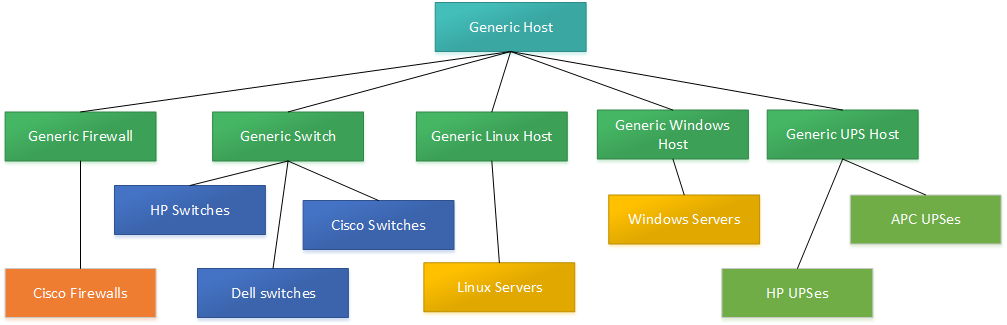
\includegraphics[scale=0.5]{img/host}
    \caption{Oversikt over host generic plassering}
    \label{hostfigur}
\end{figure}

I Figur \ref{hostgroupfigur} ser vi hvilke hostgroups de forskjellige hostene skal være medlem av.

\begin{figure}[H]
    \centering
    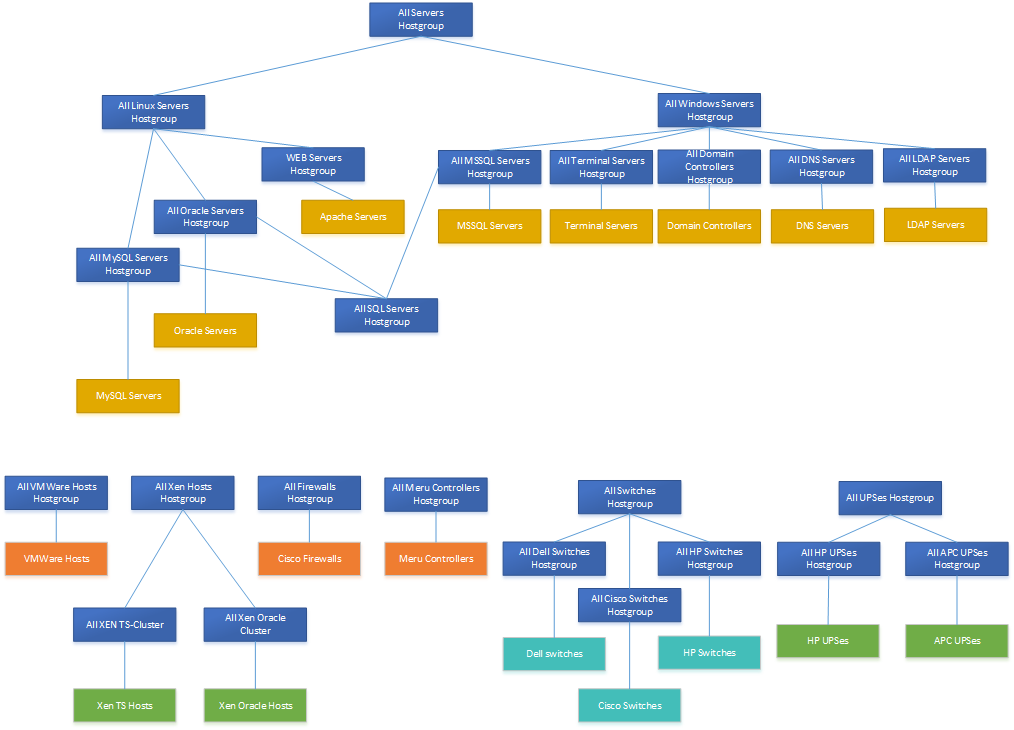
\includegraphics[scale=0.5]{img/hostgroups}
    \caption{Oversikt over hosts hostgroupplassering}
    \label{hostgroupfigur}
\end{figure}

\section{Legge til mange host-objekter}
I utrullingsfaser vil det være naturlig å legge til mange hosts på den gang. Ved å bruke "gen.bash"-scriptet spares tid samtidig som scriptet sørger for å generere hostfilene syntaktisk korrekte.

Scriptet genererer host-objekter med atributtene  ``hostname'', ``address'', ``hostgroup'' og ``generic''. Host-objekter uten hostgroup eller generic supplert, vil få standardverdier definert, mens hostname og address er obligatrisk, og det gis en feilmelding om disse er utelatt.

Eksempelet under viser hvordan scriptet kjøres og at linjenummer skrives ut dersom informasjon som er obligatorsk mangler.
\begin{lstlisting}
monkey@hig1:~/script$ vim servers.csv
monkey@hig1:~/script$ ./gen.bash servers.csv

	Generating hosts from servers.csv into working directory

	Hostname and Address are mandatory.
	Missing for host on line nr: 4
	Missing for host on line nr: 6
	Missing for host on line nr: 7
	Missing for host on line nr: 8

	Done
	Successfully created 4 hosts
	4 hosts where not created because of errors.
monkey@hig1:~/script$ ls
gen.bash  servers.csv  test1.cfg  test2.cfg  test3.cfg  test4.cfg
monkey@hig1:~/script$
\end{lstlisting}

Koden under viser hvordan servers.csv er bygget opp. Inneholder også feil for å vise hva som skjer dersom informasjonen ikke er korrekt.
\begin{lstlisting}
10.0.0.1,test1,windows;,generic1
10.0.0.1,test2,,jekrjekr
10.0.0.1,test3
,,,
10.0.0.1,test4
1,
,
,
\end{lstlisting}

Kildekoden til scriptet ligger i Vedlegg \ref{gen.bash}.

\section{Forventet nedtid}
Tilfeller kan forekomme hvor en server må tas ut av drift på grunn av vedlikehold. I Icinga er det ikke nødvendig å fjerne denne fra konfigurasjonen, for å unngå at varslingsmelding blir sendt ut. I både Icinga Web og Icinga Classic har man mulighet til å bruke en funksjon som kalles ''Schedule Downtime''. Her blir nedetidens start og slutt definert.

I den nedetidsperioden vil Icinga nekte varslingsmelding i å bli sendt ut. Når nedetidsperioden er ferdig, eller denne blir utført før avtalt tid, vil kontaktene som skal bli varslet få en melding om at nedetid er over, og Icinga vil ikke lengre holde igjen varlser.

\section{Stoppe varsling}
acknowledge, stopper gjenvarsling??
\section{Autentisering mot Active Directory} 
LDAP-autentisering brukes for å styre hvem som skal ha tilgang til web-grensesnittene, ved hjelp av grupper og brukere i Active Directory. Dette er støttet direkte i Icinga Web, men må konfigureres på andre måter for Icinga Classic. Det kan opprettes en sikkerhetsgruppe i AD som inkluderer medlemmene som skal få tilgang. Alle som er med i denne gruppen vil få tilgang til Icinga Web, der det også kan defineres hvilken informasjon hver bruker skal se. 

Selve LDAP-binden gjøres via PHP-modulen “php-ldap”. Når en bruker logger inn sjekkes først AD, dersom brukeren ikke finnes der, vil Icinga-web prøve sin egen database over brukere. Hvis brukeren finnes her og passordet er riktig vil brukeren bli logget inn. Når brukeren har logget inn for første gang via AD, vil brukeren bli lagret i Icinga Web-databasen. Om brukeren endrer passord i Icinga Web vil uansett AD først bli spurt før Icinga Web spør om passordet er riktig i sin egen database

Icinga classic autentiserer mot AD gjennom modulene ldap og authnz\_ldap.

/etc/apache2/conf.d/
\begin{lstlisting}
        AuthName "Authentication"
        AuthType Basic
        AuthBasicProvider ldap
        AuthLDAPURL
"ldap://10.60.0.22:3268/dc=monkey,dc=local?samAccountName?sub?(objectClass=person)"
        AuthLDAPBindDN "flash@monkey.local"
        AuthLDAPBindPassword "Bachel0r"
        require ldap-group CN=icinga-login, OU=icinga, DC=monkey, DC=local
\end{lstlisting}

/usr/share/icinga-web/app/modules/AppKit/config/auth.xml
\begin{lstlisting}
  <ae:parameter name="ldap_allow_anonymous">false</ae:parameter>
            <ae:parameter name="ldap_dsn">ldap://10.60.0.22</ae:parameter>
            <ae:parameter name="ldap_start_tls">false</ae:parameter>
            <ae:parameter name="ldap_basedn">DC=monkey,DC=local</ae:parameter>
            <ae:parameter name="ldap_binddn">icingawebauth@monkey.local</ae:parameter>
            <ae:parameter name="ldap_bindpw"><![CDATA[Password]]></ae:parameter>
            <ae:parameter name="ldap_userattr">sAMAccountName</ae:parameter>
            <ae:parameter name="ldap_filter_user"><![CDATA[(&(sAMAccountName=__USERNAME__)(memberOf=CN=icinga-login,OU=icinga,DC=monkey,DC=local))]]></ae:parameter>
        </ae:parameter>
\end{lstlisting}

\section{Kontakter og kontaktgrupper}

For å opprette en ny kontakt i Icinga meldes brukeren inn i gruppen icinga\_kontakter (se synkronisering). Den vil trenge å ha e-postadresse og telefonnummer satt.

Kontaktgrupper hentes fra OU-en icinga\_grupper der alle grupper hentes ut og opprettes i Icinga. For at en gruppe skal varsles må dette legges til på en service. For å slippe å sette opp kontakter for hver service kan en velge å sende med argumentet “gen\_service” for å generere en template som kan benyttes på tjenester som sorterer under hver av kontaktgruppene som blir opprettet.

Eksempel på generisk service som blir opprettet:
\begin{lstlisting}
define service {
    name network_services
    register 0
    use generic-service     
    notification_interval   30
    notification_period     24x7
    notification_options    w,c,r
    contact_groups          network_contact_group
}
\end{lstlisting}

Denne brukes på en Cisco firewall: 
\begin{lstlisting}
define service {
        service_description Cisco Firewall CPU Load
        use network_services
        name cisco-firewall-cpu-load
        hostgroup_name all_firewalls
        check_command check_network_component!cpu-load
}
\end{lstlisting}

Tabell med sjekker og tilhørende parametere:
\begin{table}
\begin{center}
\begin{tabular}{| l | l | l | l |}
 \hline
        \textbf{Utstyr} & \textbf{Service navn} & \textbf{Warning} & \textbf{Critical}
	\\ \hline
	APC UPS 		& UPS Capacity			& 90:	& 80: \\ \hline
	APC UPS			& Internal Temp			& 30	& 32 \\ \hline
	APC UPS			& Load				& 50	& 60 \\ \hline
	APC UPS			& Voltage In			& 225:239 & 220:245 \\ \hline
	APC UPS			& Voltage Out			& 225:239 & 220:245 \\ \hline 
	HP UPS			& Battery Time Remaining 	& 3000: & 2700: \\ \hline
	HP UPS			& Battery capacity		& 90: 	& 80: \\ \hline
	HP UPS			& Battery current		& 	& \\ \hline
	HP UPS			& Voltage In			& 225:239 & 220:245 \\ \hline 
	HP UPS			& Voltage Out			& 225:239 & 220:245 \\ \hline
	Windows Server		& Check DNS			& 0.1	& 0.2 \\ \hline
	Windows Server		& Check LDAP			& 0.05	& 0.1 \\ \hline 
	Windows Server		& All Disks			& 94\%	& 96\% \\ \hline
	Windows Server		& Disk Space			& 90\%	& 95\% \\ \hline
	Windows Server		& CPU Load			& 90	& 95 \\ \hline
	Windows Server		& Memory Usage			& 94\%	& 98\% \\ \hline
	Windows Server		& RDP-Sessions: Active		& 20	& 25 \\ \hline
	Windows Server		& RDP-Sessions: Inactive	& 15	& 20 \\ \hline
	Cisco ASA / PIX		& CPU Load			& 93	& 96 \\ \hline
	Cisco ASA / PIX		& Hardware Health		& N/A	& N/A \\ \hline
	Cisco ASA / PIX		& Memory Usage			& 93	& 96 \\ \hline
	Cisco ASA / PIX		& Failover Status		& N/A	& N/A \\ \hline
	Cisco ASA / PIX		& VPN Sessions			& 80 (\% av lisens) & 90 (\% av lisens) \\ \hline
	Dell Blade Chassis	& Dell Blade Server Health	& N/A	& N/A \\ \hline
	Dell Powerconnect	& Assets			& N/A	& N/A \\ \hline
	Dell Powerconnect	& Uptime			& N/A	& N/A \\ \hline
	Dell Powerconnect	& Fans				& N/A	& N/A \\ \hline
	Dell Powerconnect	& Power supply			& N/A	& N/A \\ \hline
	Dell Powerconnect	& Temperature			& 34	& 36 \\ \hline
	HP Procurve		& Environment Status		& N/A	& N/A \\ \hline
	MySQL			& Cache Hit			& 60: 	& 50: \\ \hline
	MySQL			& Health			& 0.1	& 0.2 \\ \hline
	MySQL			& Slow Queries			& 0.1	& 1 \\ \hline 
	MySQL			& User Connections		& 50	& 80 \\ \hline
	MSSQL			& Cache Hit			& 90:	& 80: \\ \hline
	MSSQL			& Health			& 0.05	& 0.15 \\ \hline
	MSSQL			& Lazy Writes			& 20	& 0 \\ \hline
	MSSQL			& User Connections		& 2000	& 2200 \\ \hline
	Oracle			& Cache Hit			& 93:	& 90: \\ \hline
	Oracle			& Connected Users		& 50	& 80 \\ \hline
	Oracle			& Connection Time		& 0.1	& 0.2 \\ \hline
	Oracle			& Free Tablespace		& 5:	& 2: \\ \hline
\end{tabular}
\label{objekt_varsling}
\end{center}
\end{table}

\section{Backup-rutiner}
I Tabell \ref{backup}, vises viktige filer og mapper for overvåkningsløsningen. Disse bør integreres i en backup av Icinga-serveren.
\begin{table} \label{backup}
\begin{center}
\begin{tabular}{| p{8cm} | p{8cm} |}
 \hline
        \textbf{Filbane} & \textbf{Inneholder}
	\\ \hline
	/etc/icinga/						& Alle konfigurasjonsfiler for Icinga \\ \hline
	/usr/lib/nagios/plugins/				& Alle plugin-er \\ \hline
	/etc/nagios-plugins/config				& Konfigurasjon for default plugins \\ \hline
	/root/Scripts						& Lokale script. \\ \hline
	/etc/snmp 						& Konfigurasjon for snmptt \\ \hline
	/etc/default/snmp 					& Konfigurasjon for at snmpd starter snmptrapd \\ \hline
	/etc/sysconfig/icinga					& Konfigurasjon for environment variabler \\ \hline
	/usr/lib/oracle/11.2/client64/network/
	admin/tnsnames.ora					& Konfigurasjon for oracle-instanser \\ \hline
	/etc/init.d/carbon-cache				& Init script for grafprosessering gjennom graphite \\ \hline
	/etc/init.d/metricinga					& Init script for prosessering av perfdata fra Icinga \\ \hline
	/opt/graphite/						& Konfigurasjon og data for genering av grafer  \\ \hline
\end{tabular}
\end{center}
\end{table}
I tilegg bruker Icinga Classic og Icinga Web hver sine databaser, kalt ''icinga'' og ''icinga\_web''. Graphite bruker også en database, som heter ''graphite''.


% Biblography

\clearpage
\bibliographystyle{plain}
\bibliography{rapport}
\addcontentsline{toc}{section}{Referanser}
\clearpage

% Appendixes

\begin{appendices}
\section{Arbeidslogg}
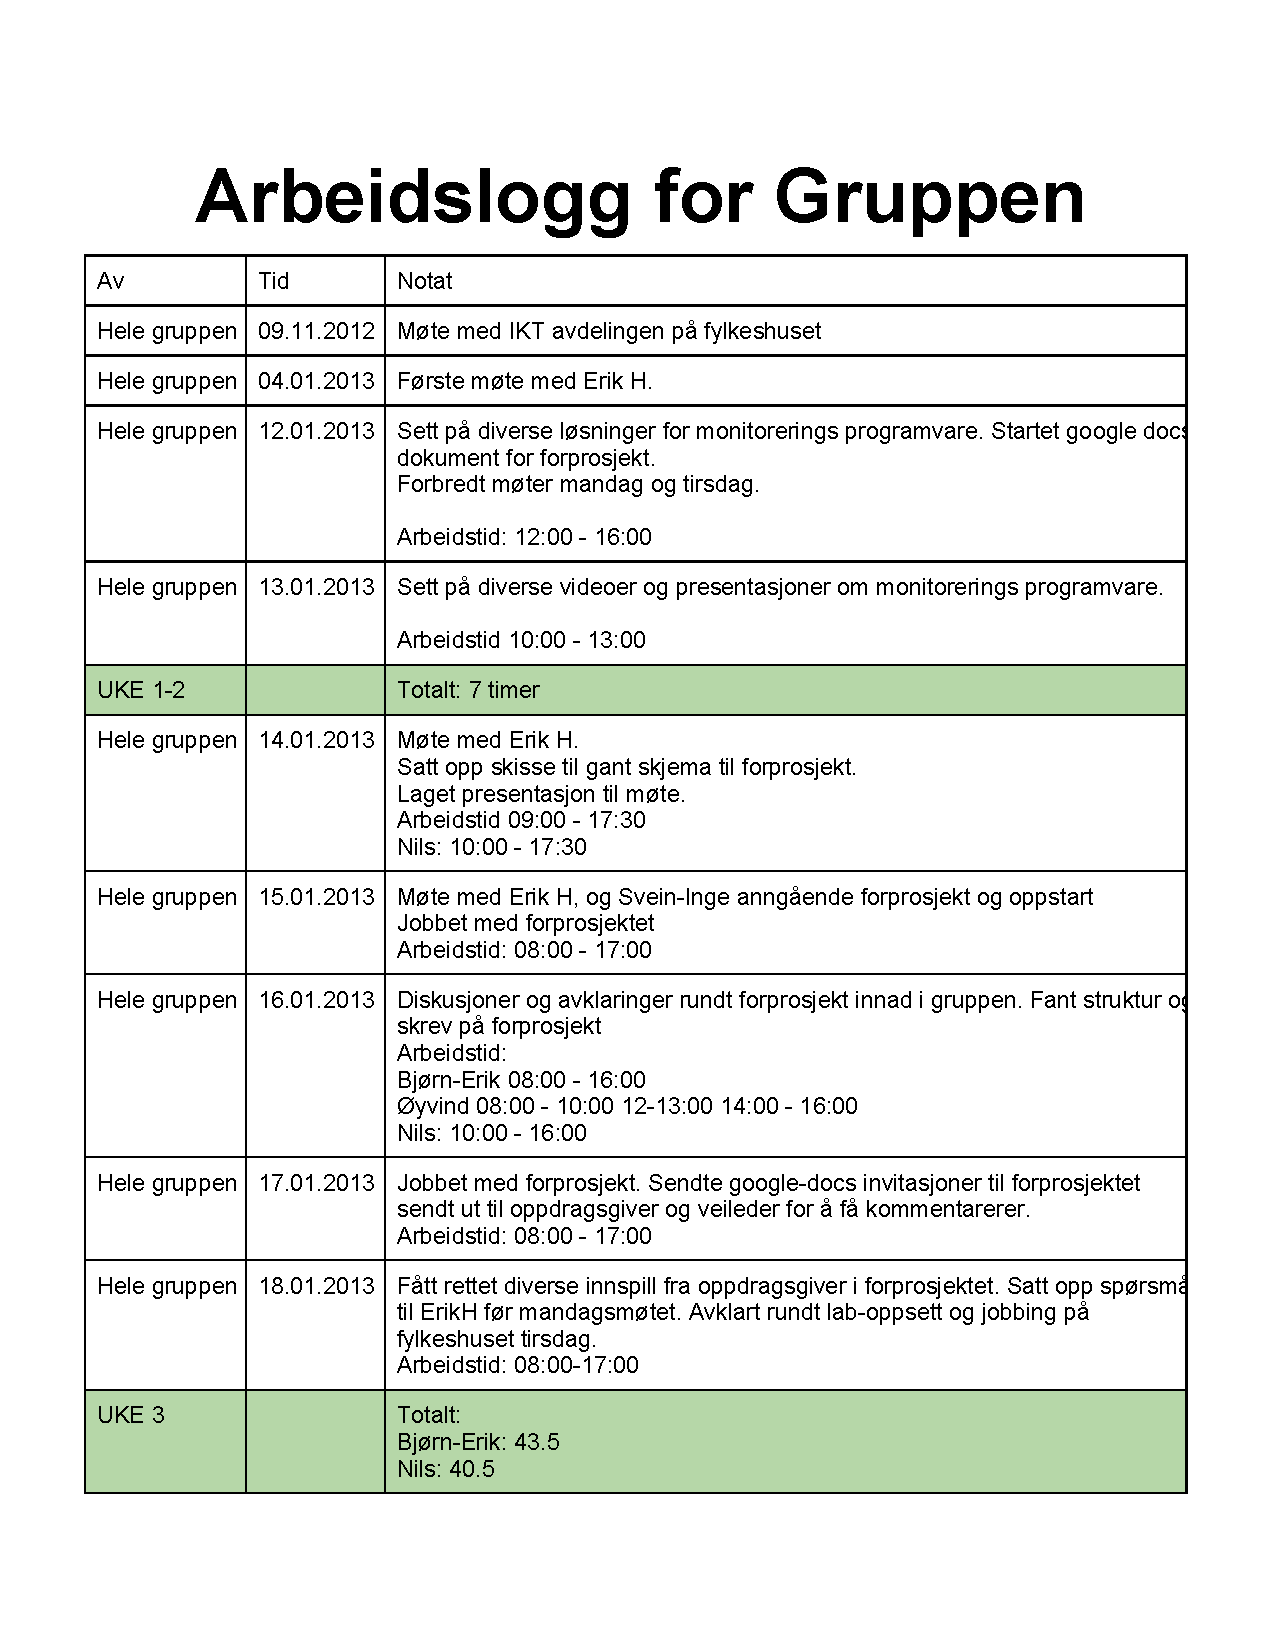
\includepdf[pages=-]{vedlegg/GruppeLogg.pdf}

\section{Møtereferater}
I dette vedlegget ligger møtereferater fra prosjektperioden.

\section{Presentasjoner}
I dette vedlegget ligger presentasjoner som ble holdt for IKT avdelingen gjennom prosjektet.

\includepdf[pages=-,landscape=true]{vedlegg/15_01_2013forprosjektmote.pdf}

\includepdf[pages=-,landscape=true]{vedlegg/29_01_2013Icinga.pdf}

\includepdf[pages=-,landscape=true]{vedlegg/05_03_2013ServerogInfrastruktur.pdf}

\section{Dokumenter}
I dette vedlegget finnes:\\ 
\indent Kartlegging av behov, som ble laget av MonKey og utredet sammen med IKT-avdelingen.\\
\indent Opplæringsdokument som ble gjennomgått sammen med Oppdragsgiver og Teknisk kontakt ved slutten av prosjektperioden.

\includepdf[pages=-, pagecommand={\label{kartlegging}}]{vedlegg/kartlegging}
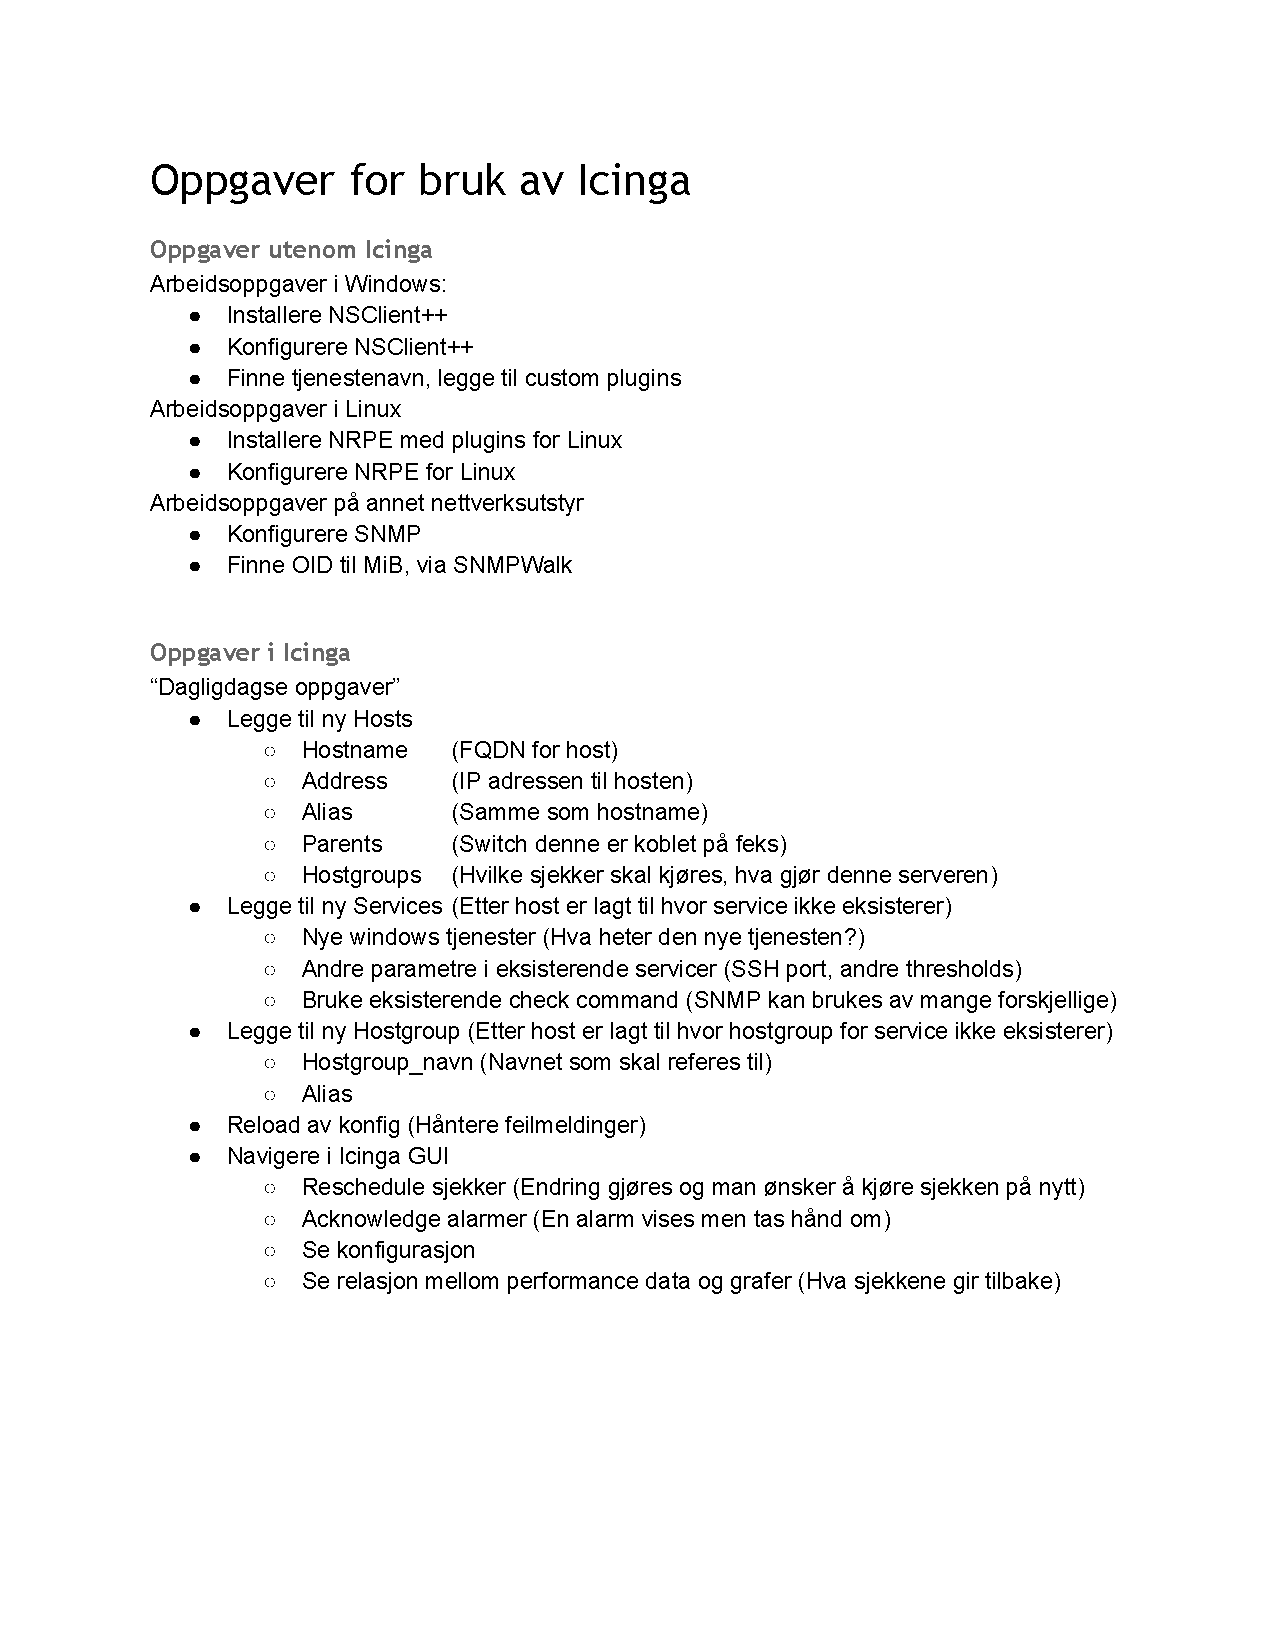
\includepdf[pages=-, pagecommand={\label{opplaering}}]{vedlegg/Opplaering}

\section{Statusrapporter}
I dette vedlegget finnes statusrapporter skrevet for hver iterasjon.
\modifiedincludepdf{-}{status1}{vedlegg/status/status1.pdf}
\modifiedincludepdf{-}{status2}{vedlegg/status/status2.pdf}


\includepdf[pages=-]{vedlegg/status/status1.pdf}

\includepdf[pages=-]{vedlegg/status/status2.pdf}

\includepdf[pages=-]{vedlegg/status/status3.pdf}

\includepdf[pages=-]{vedlegg/status/status4.pdf}

\includepdf[pages=-]{vedlegg/status/status5.pdf}
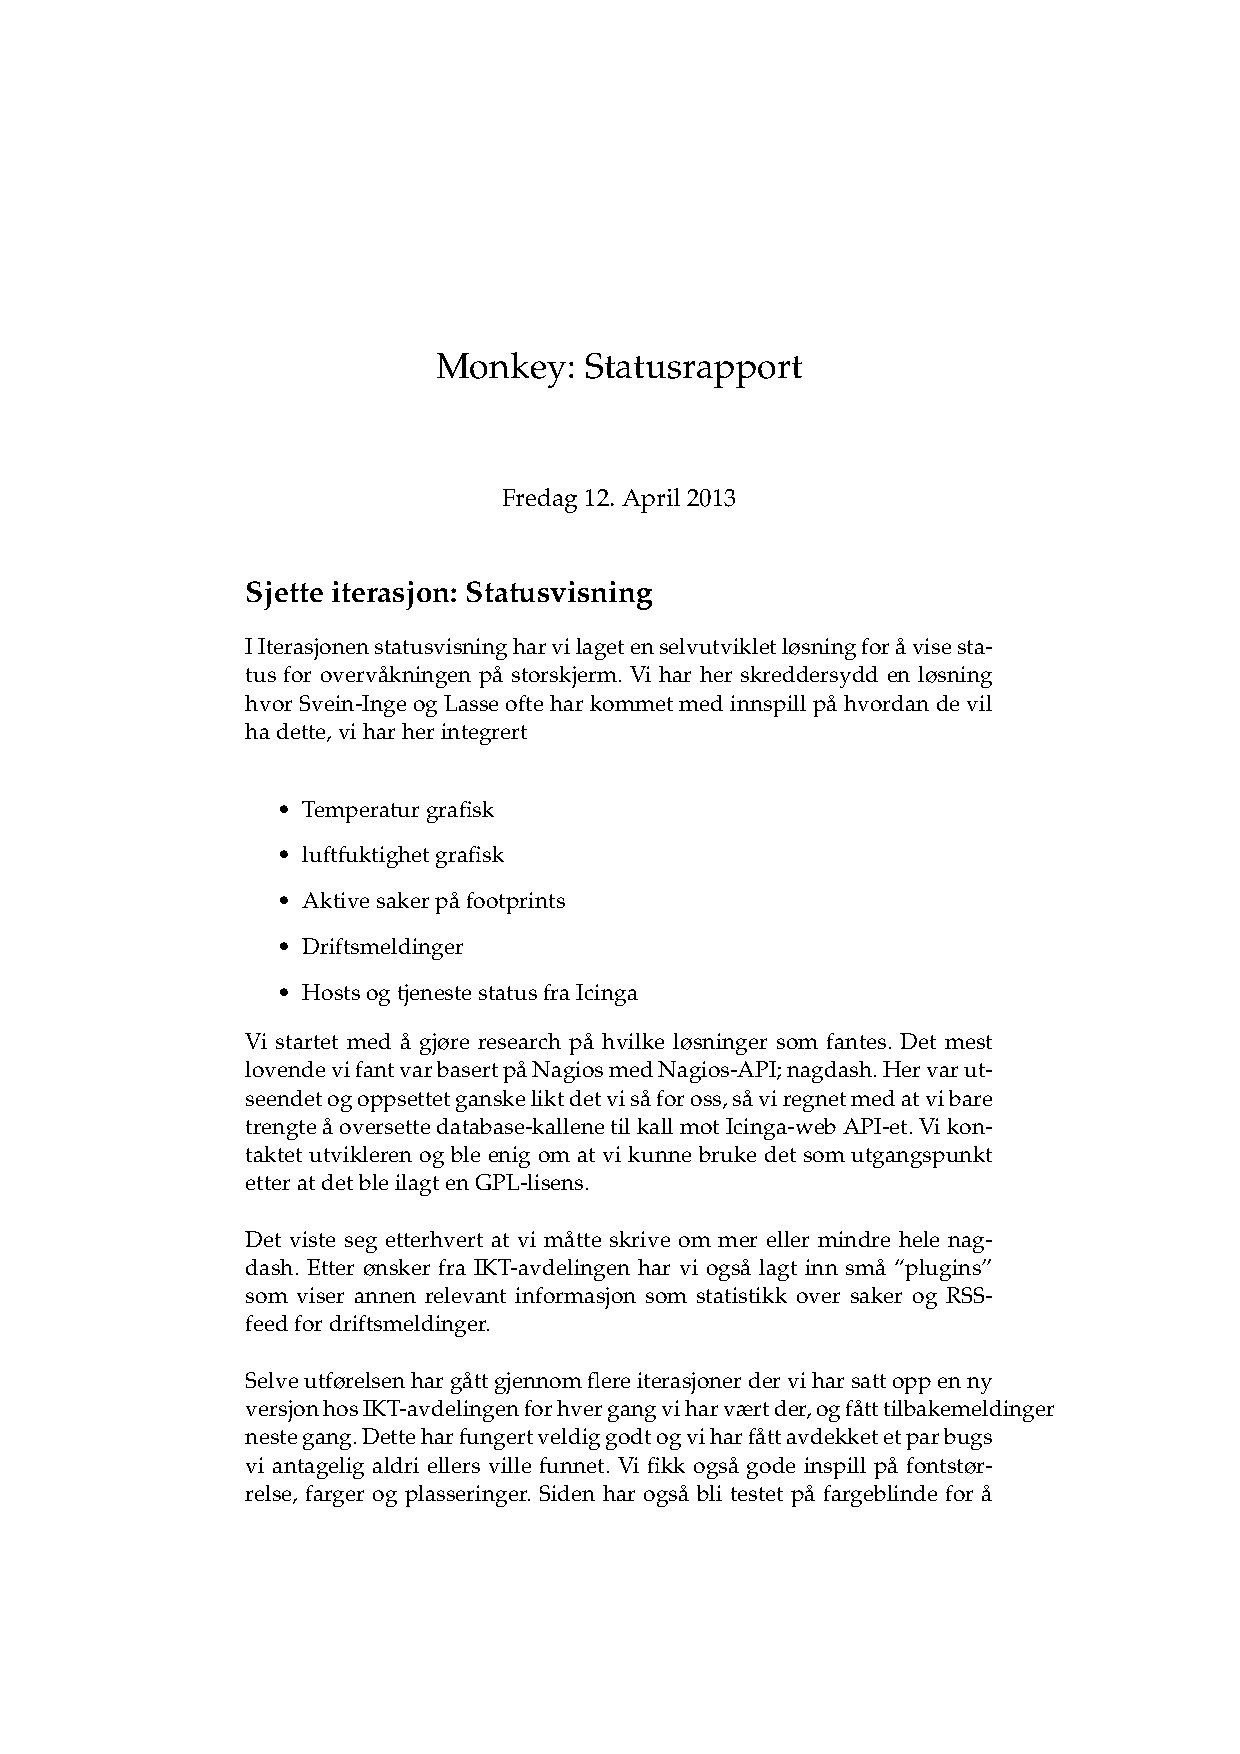
\includepdf[pages=-]{vedlegg/status/status6.pdf}

\section{Forprosjekt}
I dette vedlegget finnes forprosjektet for MonKey

\includepdf[pages=-]{../forprosjekt.pdf}

\section{Kildekode}
Selvskrevene kildekode er lagt ved under dette vedlegget. Innholder plugins og generering av hosts script.

\begin{changemargin}{-1cm}{-1cm}
\lstinputlisting[language=Bash, label={gen.bash}]{vedlegg/script/gen.bash}
\lstinputlisting[language=Perl, label={ad_sync.pl}]{vedlegg/script/ad_sync.pl}
\end{changemargin}
%\end{lstlisting}

\section{Epost}
Eposter av relevans for rapporten

\section{test}

\end{appendices}







\end{document}
